% =============================================================================
% Sección 12 del informe del proyecto: Descripción del Proyecto -- Fase 3
%
% Uso: en el documento principal, antes de \end{document}, escribir
%         % =============================================================================
% Sección 12 del informe del proyecto: Descripción del Proyecto -- Fase 3
%
% Uso: en el documento principal, antes de \end{document}, escribir
%         % =============================================================================
% Sección 12 del informe del proyecto: Descripción del Proyecto -- Fase 3
%
% Uso: en el documento principal, antes de \end{document}, escribir
%         % =============================================================================
% Sección 12 del informe del proyecto: Descripción del Proyecto -- Fase 3
%
% Uso: en el documento principal, antes de \end{document}, escribir
%         \input{seccion_fase3}
% Requiere solo el paquete graphicx (ya usado en las secciones anteriores).
% Las tablas y figuras de resultados se generan con
%         python experiments/report.py
% en el archivo fase3_resultados.tex (se incluye al final de esta sección).
% =============================================================================

\section{Descripción del Proyecto -- Fase 3}

\subsection{Objetivo de la fase}

En la Fase 2 se construyó el núcleo de ComplexNet API y se validó con tres nodos en contenedores
Docker dentro de un mismo computador. La Fase 3 convierte ese núcleo en una plataforma utilizable:
se ejecuta sobre \textbf{tres computadores físicos} conectados por una red local, ofrece una
\textbf{API documentada para desarrolladores}, incluye \textbf{tres aplicaciones descentralizadas}
construidas sobre ella, un \textbf{panel de monitoreo} del clúster y una \textbf{evaluación
experimental} de latencia, escalabilidad, disponibilidad, tolerancia a fallos y estrategias de
asignación de tareas.

\subsection{Qué se agregó respecto a la Fase 2}

El núcleo (mensajes JSON sobre UDP, descubrimiento por \emph{beacons}, detección de fallos por
silencio, reasignación de tareas y reloj lógico de Lamport) se mantiene. Lo nuevo es lo siguiente:

\begin{table}[htbp]
\centering
\small
\begin{tabular}{|p{0.2\textwidth}|p{0.33\textwidth}|p{0.33\textwidth}|}
\hline
\textbf{Aspecto} & \textbf{Fase 2} & \textbf{Fase 3} \\ \hline
Despliegue & Tres contenedores Docker en un computador, red virtual & Tres computadores físicos en una red local real \\ \hline
Descubrimiento & \emph{Broadcast} a una subred fija de Docker & Detección automática de la subred y vecinos semilla por IP \\ \hline
Uso del sistema & Script de demostración & API para desarrolladores y manual \\ \hline
Aplicaciones & Una tarea de regresión lineal de ejemplo & Tres aplicaciones descentralizadas \\ \hline
Monitoreo & Terminal y un archivo JSON por nodo & Panel web en vivo con alertas \\ \hline
Planificación & Una función de aptitud $F(i,j)$ & Seis estrategias intercambiables en caliente \\ \hline
Capacidad del nodo & Sin límite de tareas simultáneas & Ranuras de ejecución (\emph{slots}) y cola \\ \hline
Validación & Pruebas funcionales (42) & Pruebas (66) y experimentos con informe \\ \hline
\end{tabular}
\caption{Cambios de la Fase 3 respecto a la Fase 2.}
\label{tab:fase2-fase3}
\end{table}

\subsection{Despliegue en tres computadores}

\paragraph{¿Cómo se conectan los computadores?}
Los tres equipos se conectan a la \textbf{misma red local} (mismo Wi-Fi o router; también sirve el
punto de acceso de un celular). No se usa ningún servidor central ni se necesita internet: cada
nodo envía los mensajes directamente a los demás mediante \textbf{UDP sobre IP}, por el puerto
\texttt{9999}. El panel web usa el puerto \texttt{8000} (TCP) y es solo para observar y administrar.

\begin{table}[htbp]
\centering
\small
\begin{tabular}{|c|c|p{0.5\textwidth}|}
\hline
\textbf{Equipo} & \textbf{Nodo} & \textbf{Qué ejecuta} \\ \hline
Computador 1 & \texttt{nodo-01} & Un nodo, las aplicaciones y los experimentos \\ \hline
Computador 2 & \texttt{nodo-02} & Solo el nodo \\ \hline
Computador 3 & \texttt{nodo-03} & Solo el nodo \\ \hline
\end{tabular}
\caption{Distribución de nodos en los computadores.}
\label{tab:tres-pcs}
\end{table}

\paragraph{Descubrimiento en la red real.}
\begin{enumerate}
\item Cada nodo emite cada 2 s un mensaje \texttt{RESOURCE\_BEACON} por \emph{broadcast} UDP, es decir,
a la dirección que reciben todos los equipos de la subred. El nodo calcula esa dirección a partir de
su propia IP y máscara de red (opción \texttt{--broadcast auto}).
\item El \emph{beacon} informa el identificador del nodo, su IP, su CPU libre, su memoria libre, su ancho
de banda y cuántas tareas tiene en curso.
\item Al recibir el \emph{beacon} de un nodo desconocido, el receptor lo registra en su \texttt{PeerTable}
y le responde con un \emph{beacon} directo. Así, basta con que uno de los dos oiga al otro para que
ambos se descubran.
\item Si la red bloquea el \emph{broadcast} (algunas redes institucionales lo filtran), cada nodo puede
iniciarse con las IP de sus vecinos (\texttt{--peers}) y los mensajes viajan de forma directa. Otra
alternativa es conectar los tres equipos al punto de acceso de un celular.
\end{enumerate}

\paragraph{Mensajes del protocolo.}
Todos los mensajes son JSON con un encabezado (identificador único, emisor, tipo, marca de tiempo y
reloj de Lamport) y una carga útil. El tamaño máximo es de 60 KB, de modo que cada mensaje cabe en un
datagrama UDP.

\begin{table}[htbp]
\centering
\small
\begin{tabular}{|l|p{0.55\textwidth}|}
\hline
\textbf{Mensaje} & \textbf{Función} \\ \hline
\texttt{RESOURCE\_BEACON} & Presencia y recursos del nodo (cada 2 s) \\ \hline
\texttt{PING} / \texttt{PONG} & Medición de la latencia (RTT) entre dos nodos \\ \hline
\texttt{TASK\_SUBMIT} & Envío de una tarea al nodo elegido \\ \hline
\texttt{TASK\_ACK} & Confirmación de recepción de la tarea \\ \hline
\texttt{TASK\_RESULT} & Resultado de la tarea o error \\ \hline
\texttt{ALERT} & Alerta difundida a todos los nodos (Fase 3) \\ \hline
\end{tabular}
\caption{Mensajes intercambiados entre los nodos.}
\label{tab:mensajes}
\end{table}

\paragraph{Puesta en marcha.}
Cada computador ejecuta un único comando, que crea el entorno de Python, instala las dependencias,
abre el puerto en el cortafuegos y arranca el nodo:

\begin{verbatim}
.\scripts\start_node.ps1 -Id nodo-02
\end{verbatim}

\subsection{API para desarrolladores}

La clase \texttt{Node} es la puerta de entrada: oculta el descubrimiento, la planificación, la
comunicación y la recuperación ante fallos. Una aplicación necesita pocas líneas:

\begin{verbatim}
from complexnet import Node, Task

with Node("nodo-01", broadcast_address="auto") as node:
    node.wait_for_peers(2)
    tarea = Task("regresion_lineal", {"n_samples": 10000},
                 requirements={"cpu": 1, "memory": 256})
    resultado = node.submit(tarea)      # el planificador elige el nodo
\end{verbatim}

\begin{table}[htbp]
\centering
\small
\begin{tabular}{|p{0.3\textwidth}|p{0.6\textwidth}|}
\hline
\textbf{Método} & \textbf{Descripción} \\ \hline
\texttt{connect()}, \texttt{disconnect()} & Une el nodo a la red o lo detiene (también como \texttt{with}) \\ \hline
\texttt{wait\_for\_peers(n)} & Espera hasta tener $n$ vecinos activos \\ \hline
\texttt{submit(tarea)} & Envía una tarea y devuelve su resultado (o la tarea, sin esperar) \\ \hline
\texttt{map(nombre, lista)} & Una tarea por elemento; devuelve los resultados en orden \\ \hline
\texttt{map\_tasks(...)} & Igual que \texttt{map}, pero devuelve las tareas con sus tiempos y el nodo ejecutor \\ \hline
\texttt{broadcast(tipo, datos)} & Envía un mensaje a todos los vecinos activos \\ \hline
\texttt{raise\_alert(nivel, texto)} & Registra una alerta y la difunde a toda la red \\ \hline
\texttt{on\_event(funcion)} & Ejecuta una función por cada evento del nodo (fallos, tareas, descubrimiento) \\ \hline
\texttt{set\_strategy(nombre)} & Cambia la estrategia de asignación en caliente \\ \hline
\texttt{simulate\_failure(s)} & Simula una caída del nodo durante $s$ segundos (pruebas) \\ \hline
\texttt{status()} & Estado completo: recursos, vecinos, tareas, alertas y métricas \\ \hline
\end{tabular}
\caption{Métodos principales de la API.}
\label{tab:api}
\end{table}

Una \texttt{Task} lleva un nombre, sus parámetros y requisitos (CPU libre mínima, memoria mínima y,
opcionalmente, una lista de nodos permitidos). Los tipos de tarea disponibles son los siguientes:

\begin{table}[htbp]
\centering
\small
\begin{tabular}{|l|p{0.55\textwidth}|}
\hline
\textbf{Tarea} & \textbf{Descripción} \\ \hline
\texttt{regresion\_lineal} & Regresión lineal completa en un nodo (Fase 2) \\ \hline
\texttt{normal\_equations} & Estadísticos de un fragmento de datos para la regresión distribuida \\ \hline
\texttt{evaluate\_model} & Evaluación de un modelo sobre un fragmento de datos \\ \hline
\texttt{monte\_carlo\_pi} & Estimación de $\pi$ por el método de Monte Carlo \\ \hline
\texttt{word\_count} & Conteo de palabras de un fragmento de texto \\ \hline
\end{tabular}
\caption{Tipos de tarea incluidos.}
\label{tab:tareas}
\end{table}

Agregar una tarea nueva consiste en escribir una función de Python que reciba un diccionario y
devuelva otro, y registrarla en el módulo de ejecutores. La referencia completa está en el manual del
desarrollador (\texttt{docs/api/MANUAL\_DESARROLLADOR.md}).

\subsection{Aplicaciones descentralizadas}

Las tres aplicaciones usan únicamente la API anterior; ninguna depende de un servidor central.

\subsubsection{Aplicación 1: monitoreo distribuido con alertas}

Vigila el clúster con la información que ya circula en los \emph{beacons} y genera alertas que se
\textbf{difunden a todos los nodos}, de modo que cada nodo conserva su propio registro de alertas.

\begin{itemize}
\item \textbf{Crítica:} un nodo pasa a \texttt{OFFLINE}.
\item \textbf{Informativa:} un nodo vuelve a estar \texttt{ONLINE}.
\item \textbf{Advertencia:} CPU libre menor a un umbral, memoria libre menor a un umbral o latencia
mayor a un umbral (configurables).
\end{itemize}

Además guarda una serie de tiempo con la CPU, la memoria y la latencia de cada nodo, y las alertas
aparecen en el panel web.

\subsubsection{Aplicación 2: procesamiento distribuido}

Realiza dos trabajos de tipo \emph{map-reduce} repartidos por la red:

\begin{enumerate}
\item \textbf{Análisis de archivos:} los archivos de texto de una carpeta se parten en fragmentos; cada
nodo cuenta las palabras de su fragmento (\emph{map}) y el nodo coordinador combina los conteos
(\emph{reduce}).
\item \textbf{Cálculo colaborativo:} estimación de $\pi$ por Monte Carlo. Cada nodo lanza puntos al azar
en el cuadrado unidad y cuenta los que caen dentro del círculo; con el total se obtiene
$\pi \approx 4 \cdot \mathrm{dentro} / \mathrm{total}$.
\end{enumerate}

Si un nodo cae durante el trabajo, sus fragmentos se reasignan y el resultado no cambia.

\subsubsection{Aplicación 3: inteligencia artificial distribuida}

Entrena una \textbf{regresión lineal múltiple} repartiendo los datos entre los nodos. La idea es que
la solución de mínimos cuadrados se puede calcular a partir de sumas parciales. Si el conjunto de
datos se divide en fragmentos $(X_k, y_k)$, cada nodo calcula $X_k^{\top}X_k$ y $X_k^{\top}y_k$ de su
fragmento y el coordinador los suma y resuelve:

\begin{equation}
\hat{w} = \Bigl(\sum_k X_k^{\top}X_k\Bigr)^{-1} \sum_k X_k^{\top}y_k
\end{equation}

El resultado es exactamente el de entrenar con todos los datos en un solo equipo. Cada fragmento se
genera dentro del nodo que lo procesa a partir de una semilla, por lo que por la red solo viajan
parámetros pequeños y estadísticos. El modelo se evalúa después en fragmentos nuevos, también
repartidos, calculando el coeficiente de determinación
$R^2 = 1 - \mathrm{SSE}/\mathrm{SST}$. Si un nodo falla durante el entrenamiento, su fragmento se
reasigna a otro y los pesos finales son los mismos.

\begin{table}[htbp]
\centering
\small
\begin{tabular}{|p{0.28\textwidth}|p{0.62\textwidth}|}
\hline
\textbf{Requisito del taller} & \textbf{Cómo se cumple} \\ \hline
Distribución de datos & Fragmentos generados en cada nodo a partir de una semilla \\ \hline
Asignación de recursos & El planificador reparte cada fragmento según CPU, memoria, ancho de banda, latencia, reputación y carga \\ \hline
Información intercambiada & Estadísticos $X_k^{\top}X_k$, $X_k^{\top}y_k$ y sumas de cuadrados, no los datos \\ \hline
Métricas & Error de los pesos, $R^2$, MSE, tiempos y fragmentos por nodo \\ \hline
Tolerancia a fallos & Reasignación automática del fragmento del nodo caído \\ \hline
\end{tabular}
\caption{Aplicación de inteligencia artificial: cumplimiento de los requisitos.}
\label{tab:ia}
\end{table}

\subsection{Estrategias de asignación de tareas}

El planificador de la Fase 2 implementa la función de aptitud del diseño (sección 9):

\begin{equation}
F(i,j) = 0.40\,C' + 0.40\,M' + 0.10\,B' + 0.05\,R - 0.05\,(1 - L')
\end{equation}

donde $C'$, $M'$, $B'$ y $L'$ son la CPU libre, la memoria libre, el ancho de banda y la latencia
(esta última con normalización inversa) normalizados entre los candidatos, y $R$ es la reputación del
nodo. Al probarla en los experimentos se observó un problema: la normalización min-max convierte
diferencias mínimas entre nodos casi idénticos (por ejemplo, 1\,\% de CPU) en diferencias de 0 a 1, y
la función no conoce cuántas tareas tiene ya cada nodo, así que podía enviar todas las tareas al mismo
nodo.

Para resolverlo se agregó la variante \texttt{weighted\_load}, que usa por defecto:

\begin{itemize}
\item \textbf{Normalización robusta:} $x' = (x - \min x) / \max(\max x - \min x,\ \delta)$, donde
$\delta$ es un rango mínimo significativo ($\delta_C = 20$ puntos de CPU libre, $\delta_M = \delta_B = 20\,\%$
del mayor valor y $\delta_L = 5$ ms). Las diferencias de ruido ya no se amplifican.
\item \textbf{Término de carga:} se resta $0.30\,Q'$, donde $Q'$ es el número de tareas en curso del
nodo (incluidas las que el propio coordinador le acaba de enviar) normalizado entre los candidatos; los
pesos de CPU y memoria bajan a 0.25 para que la suma siga siendo 1.
\end{itemize}

\begin{equation}
F_{L}(i,j) = 0.25\,C' + 0.25\,M' + 0.10\,B' + 0.05\,R - 0.05\,(1 - L') - 0.30\,Q'
\end{equation}

Además se implementaron cuatro estrategias de referencia para compararlas:

\begin{table}[htbp]
\centering
\small
\begin{tabular}{|l|p{0.6\textwidth}|}
\hline
\textbf{Estrategia} & \textbf{Criterio} \\ \hline
\texttt{weighted} & $F(i,j)$ del diseño \\ \hline
\texttt{weighted\_load} & $F_L(i,j)$: robusta y con carga (por defecto) \\ \hline
\texttt{least\_loaded} & El nodo con menos tareas en curso \\ \hline
\texttt{lowest\_latency} & El nodo con menor latencia medida \\ \hline
\texttt{round\_robin} & Reparto cíclico entre los candidatos aptos \\ \hline
\texttt{random} & Un candidato apto al azar \\ \hline
\end{tabular}
\caption{Estrategias de asignación implementadas.}
\label{tab:estrategias-lista}
\end{table}

En todas, el conjunto de candidatos se filtra primero con los requisitos de la tarea
($C_i \geq C_{\mathrm{req}}$ y $M_i \geq M_{\mathrm{req}}$) y solo se consideran los nodos activos.

\paragraph{Capacidad de los nodos.}
Cada nodo ejecuta como máximo \texttt{slots} tareas a la vez (2 por defecto); las demás esperan en cola.
Esto modela un computador con CPU limitada y hace que el reparto de carga sea relevante.

\subsection{Panel de monitoreo del clúster}

Cada nodo sirve una página web (\texttt{http://IP-DEL-NODO:8000}) que muestra, en tiempo real, los
nodos del clúster con su estado, CPU, memoria y latencia, la evolución de la latencia, las tareas y sus
resultados, las alertas y el registro de eventos. El mismo servicio expone una API HTTP: consulta del
estado (\texttt{GET /status}, \texttt{GET /events}), envío de tareas (\texttt{POST /tasks}) y
administración para los experimentos (\texttt{POST /admin/fail} para simular una caída remota y
\texttt{POST /admin/strategy} para cambiar la estrategia).

\subsection{Metodología experimental}

Los experimentos se ejecutan con \texttt{experiments/run\_experiments.py} desde el computador 1 y el
informe se genera con \texttt{experiments/report.py} a partir de los archivos CSV resultantes. La carga
de trabajo son tareas de Monte Carlo (intensivas en CPU), y cada medición se repite varias veces para
reportar la media y la desviación estándar. Se evalúan:

\begin{itemize}
\item \textbf{Latencia:} RTT de \texttt{PING}/\texttt{PONG} y tiempo de una tarea mínima.
\item \textbf{Tiempo de descubrimiento:} desde que arranca un nodo nuevo hasta conocer a los demás.
\item \textbf{Escalabilidad:} el mismo lote con 1, 2 y 3 nodos (aceleración) y cargas crecientes.
\item \textbf{Estrategias de asignación:} el mismo lote heterogéneo con las seis estrategias.
\item \textbf{Tolerancia a fallos:} un nodo cae a mitad de un lote y se mide la detección, la
recuperación y el porcentaje de tareas completadas.
\item \textbf{Disponibilidad:} se envía una tarea de sondeo cada 0.5 s mientras un nodo falla.
\end{itemize}

Las fallas se inyectan con el endpoint \texttt{/admin/fail} del nodo víctima, que deja de enviar y
recibir mensajes durante unos segundos, lo que equivale a una caída o a una desconexión de la red.

\subsection{Resultados experimentales}

Las tablas y gráficas de esta sección se generan automáticamente a partir de los datos medidos.

\input{fase3_resultados}

\subsection{Pruebas}

El proyecto incluye 66 pruebas automáticas (\texttt{python -m pytest tests}): 42 de las fases anteriores
(planificador, mensajes, reloj de Lamport, tabla de vecinos, detector de fallos y escenarios de
integración con tres nodos reales) y 24 de la Fase 3, que verifican:

\begin{itemize}
\item las seis estrategias y su respeto por los requisitos de la tarea;
\item la normalización robusta (sin amplificar diferencias mínimas) y el ejemplo numérico del diseño;
\item que la suma de los estadísticos de los fragmentos equivale a la regresión sobre todos los datos;
\item la API (\texttt{map} conserva el orden, el requisito de nodos, el cambio de estrategia, \texttt{on\_event});
\item que una alerta llega al registro de todos los nodos;
\item que un nodo caído pasa a \texttt{OFFLINE}, se recupera y que sus tareas se reasignan;
\item que las ranuras limitan la ejecución simultánea y la detección de la subred.
\end{itemize}

\subsection{Qué se puede demostrar en la sustentación}

\begin{itemize}
\item Tres computadores físicos descubriéndose automáticamente en la misma red.
\item El panel web mostrando los tres nodos, sus recursos, la latencia y las tareas en vivo.
\item Las tres aplicaciones: alertas de monitoreo, procesamiento \emph{map-reduce} y regresión
lineal distribuida.
\item La caída de un nodo durante una tarea: alerta crítica, reasignación automática y resultado
correcto.
\item El cambio de estrategia de asignación en caliente y su efecto en el reparto.
\item Las métricas y gráficas de los experimentos.
\end{itemize}

\subsection{Limitaciones}

\begin{itemize}
\item El ancho de banda de cada nodo es un valor declarado, no medido.
\item UDP no garantiza la entrega ni hay retransmisión: la pérdida de un mensaje se maneja con el
\emph{timeout} de la confirmación y la reasignación de la tarea.
\item El nodo que envía una tarea la coordina; si ese nodo cae, pierde el estado de sus tareas, porque
no hay persistencia.
\item La sincronización es un orden lógico de eventos (Lamport); no hay exclusión mutua distribuida.
\item Los \emph{endpoints} de administración no tienen autenticación (uso de laboratorio).
\item Las tareas deben ser lo bastante grandes para amortizar el costo de la comunicación.
\end{itemize}

\subsection{Conclusión de la fase}

Con esta fase se completa ComplexNet API: una red de tres computadores físicos que se descubren solos,
reparten el trabajo con reglas locales, ejecutan aplicaciones de monitoreo, procesamiento y
aprendizaje automático distribuido, detectan fallos y se recuperan sin intervención humana ni
coordinador central. La API permite a otros desarrolladores crear nuevas aplicaciones con pocas líneas,
y la evaluación experimental respalda el comportamiento del sistema en latencia, escalabilidad,
disponibilidad y tolerancia a fallos. Del análisis de las estrategias de asignación resultó una mejora
al modelo original (normalización robusta y término de carga) que evita concentrar las tareas en un
solo nodo.

% Requiere solo el paquete graphicx (ya usado en las secciones anteriores).
% Las tablas y figuras de resultados se generan con
%         python experiments/report.py
% en el archivo fase3_resultados.tex (se incluye al final de esta sección).
% =============================================================================

\section{Descripción del Proyecto -- Fase 3}

\subsection{Objetivo de la fase}

En la Fase 2 se construyó el núcleo de ComplexNet API y se validó con tres nodos en contenedores
Docker dentro de un mismo computador. La Fase 3 convierte ese núcleo en una plataforma utilizable:
se ejecuta sobre \textbf{tres computadores físicos} conectados por una red local, ofrece una
\textbf{API documentada para desarrolladores}, incluye \textbf{tres aplicaciones descentralizadas}
construidas sobre ella, un \textbf{panel de monitoreo} del clúster y una \textbf{evaluación
experimental} de latencia, escalabilidad, disponibilidad, tolerancia a fallos y estrategias de
asignación de tareas.

\subsection{Qué se agregó respecto a la Fase 2}

El núcleo (mensajes JSON sobre UDP, descubrimiento por \emph{beacons}, detección de fallos por
silencio, reasignación de tareas y reloj lógico de Lamport) se mantiene. Lo nuevo es lo siguiente:

\begin{table}[htbp]
\centering
\small
\begin{tabular}{|p{0.2\textwidth}|p{0.33\textwidth}|p{0.33\textwidth}|}
\hline
\textbf{Aspecto} & \textbf{Fase 2} & \textbf{Fase 3} \\ \hline
Despliegue & Tres contenedores Docker en un computador, red virtual & Tres computadores físicos en una red local real \\ \hline
Descubrimiento & \emph{Broadcast} a una subred fija de Docker & Detección automática de la subred y vecinos semilla por IP \\ \hline
Uso del sistema & Script de demostración & API para desarrolladores y manual \\ \hline
Aplicaciones & Una tarea de regresión lineal de ejemplo & Tres aplicaciones descentralizadas \\ \hline
Monitoreo & Terminal y un archivo JSON por nodo & Panel web en vivo con alertas \\ \hline
Planificación & Una función de aptitud $F(i,j)$ & Seis estrategias intercambiables en caliente \\ \hline
Capacidad del nodo & Sin límite de tareas simultáneas & Ranuras de ejecución (\emph{slots}) y cola \\ \hline
Validación & Pruebas funcionales (42) & Pruebas (66) y experimentos con informe \\ \hline
\end{tabular}
\caption{Cambios de la Fase 3 respecto a la Fase 2.}
\label{tab:fase2-fase3}
\end{table}

\subsection{Despliegue en tres computadores}

\paragraph{¿Cómo se conectan los computadores?}
Los tres equipos se conectan a la \textbf{misma red local} (mismo Wi-Fi o router; también sirve el
punto de acceso de un celular). No se usa ningún servidor central ni se necesita internet: cada
nodo envía los mensajes directamente a los demás mediante \textbf{UDP sobre IP}, por el puerto
\texttt{9999}. El panel web usa el puerto \texttt{8000} (TCP) y es solo para observar y administrar.

\begin{table}[htbp]
\centering
\small
\begin{tabular}{|c|c|p{0.5\textwidth}|}
\hline
\textbf{Equipo} & \textbf{Nodo} & \textbf{Qué ejecuta} \\ \hline
Computador 1 & \texttt{nodo-01} & Un nodo, las aplicaciones y los experimentos \\ \hline
Computador 2 & \texttt{nodo-02} & Solo el nodo \\ \hline
Computador 3 & \texttt{nodo-03} & Solo el nodo \\ \hline
\end{tabular}
\caption{Distribución de nodos en los computadores.}
\label{tab:tres-pcs}
\end{table}

\paragraph{Descubrimiento en la red real.}
\begin{enumerate}
\item Cada nodo emite cada 2 s un mensaje \texttt{RESOURCE\_BEACON} por \emph{broadcast} UDP, es decir,
a la dirección que reciben todos los equipos de la subred. El nodo calcula esa dirección a partir de
su propia IP y máscara de red (opción \texttt{--broadcast auto}).
\item El \emph{beacon} informa el identificador del nodo, su IP, su CPU libre, su memoria libre, su ancho
de banda y cuántas tareas tiene en curso.
\item Al recibir el \emph{beacon} de un nodo desconocido, el receptor lo registra en su \texttt{PeerTable}
y le responde con un \emph{beacon} directo. Así, basta con que uno de los dos oiga al otro para que
ambos se descubran.
\item Si la red bloquea el \emph{broadcast} (algunas redes institucionales lo filtran), cada nodo puede
iniciarse con las IP de sus vecinos (\texttt{--peers}) y los mensajes viajan de forma directa. Otra
alternativa es conectar los tres equipos al punto de acceso de un celular.
\end{enumerate}

\paragraph{Mensajes del protocolo.}
Todos los mensajes son JSON con un encabezado (identificador único, emisor, tipo, marca de tiempo y
reloj de Lamport) y una carga útil. El tamaño máximo es de 60 KB, de modo que cada mensaje cabe en un
datagrama UDP.

\begin{table}[htbp]
\centering
\small
\begin{tabular}{|l|p{0.55\textwidth}|}
\hline
\textbf{Mensaje} & \textbf{Función} \\ \hline
\texttt{RESOURCE\_BEACON} & Presencia y recursos del nodo (cada 2 s) \\ \hline
\texttt{PING} / \texttt{PONG} & Medición de la latencia (RTT) entre dos nodos \\ \hline
\texttt{TASK\_SUBMIT} & Envío de una tarea al nodo elegido \\ \hline
\texttt{TASK\_ACK} & Confirmación de recepción de la tarea \\ \hline
\texttt{TASK\_RESULT} & Resultado de la tarea o error \\ \hline
\texttt{ALERT} & Alerta difundida a todos los nodos (Fase 3) \\ \hline
\end{tabular}
\caption{Mensajes intercambiados entre los nodos.}
\label{tab:mensajes}
\end{table}

\paragraph{Puesta en marcha.}
Cada computador ejecuta un único comando, que crea el entorno de Python, instala las dependencias,
abre el puerto en el cortafuegos y arranca el nodo:

\begin{verbatim}
.\scripts\start_node.ps1 -Id nodo-02
\end{verbatim}

\subsection{API para desarrolladores}

La clase \texttt{Node} es la puerta de entrada: oculta el descubrimiento, la planificación, la
comunicación y la recuperación ante fallos. Una aplicación necesita pocas líneas:

\begin{verbatim}
from complexnet import Node, Task

with Node("nodo-01", broadcast_address="auto") as node:
    node.wait_for_peers(2)
    tarea = Task("regresion_lineal", {"n_samples": 10000},
                 requirements={"cpu": 1, "memory": 256})
    resultado = node.submit(tarea)      # el planificador elige el nodo
\end{verbatim}

\begin{table}[htbp]
\centering
\small
\begin{tabular}{|p{0.3\textwidth}|p{0.6\textwidth}|}
\hline
\textbf{Método} & \textbf{Descripción} \\ \hline
\texttt{connect()}, \texttt{disconnect()} & Une el nodo a la red o lo detiene (también como \texttt{with}) \\ \hline
\texttt{wait\_for\_peers(n)} & Espera hasta tener $n$ vecinos activos \\ \hline
\texttt{submit(tarea)} & Envía una tarea y devuelve su resultado (o la tarea, sin esperar) \\ \hline
\texttt{map(nombre, lista)} & Una tarea por elemento; devuelve los resultados en orden \\ \hline
\texttt{map\_tasks(...)} & Igual que \texttt{map}, pero devuelve las tareas con sus tiempos y el nodo ejecutor \\ \hline
\texttt{broadcast(tipo, datos)} & Envía un mensaje a todos los vecinos activos \\ \hline
\texttt{raise\_alert(nivel, texto)} & Registra una alerta y la difunde a toda la red \\ \hline
\texttt{on\_event(funcion)} & Ejecuta una función por cada evento del nodo (fallos, tareas, descubrimiento) \\ \hline
\texttt{set\_strategy(nombre)} & Cambia la estrategia de asignación en caliente \\ \hline
\texttt{simulate\_failure(s)} & Simula una caída del nodo durante $s$ segundos (pruebas) \\ \hline
\texttt{status()} & Estado completo: recursos, vecinos, tareas, alertas y métricas \\ \hline
\end{tabular}
\caption{Métodos principales de la API.}
\label{tab:api}
\end{table}

Una \texttt{Task} lleva un nombre, sus parámetros y requisitos (CPU libre mínima, memoria mínima y,
opcionalmente, una lista de nodos permitidos). Los tipos de tarea disponibles son los siguientes:

\begin{table}[htbp]
\centering
\small
\begin{tabular}{|l|p{0.55\textwidth}|}
\hline
\textbf{Tarea} & \textbf{Descripción} \\ \hline
\texttt{regresion\_lineal} & Regresión lineal completa en un nodo (Fase 2) \\ \hline
\texttt{normal\_equations} & Estadísticos de un fragmento de datos para la regresión distribuida \\ \hline
\texttt{evaluate\_model} & Evaluación de un modelo sobre un fragmento de datos \\ \hline
\texttt{monte\_carlo\_pi} & Estimación de $\pi$ por el método de Monte Carlo \\ \hline
\texttt{word\_count} & Conteo de palabras de un fragmento de texto \\ \hline
\end{tabular}
\caption{Tipos de tarea incluidos.}
\label{tab:tareas}
\end{table}

Agregar una tarea nueva consiste en escribir una función de Python que reciba un diccionario y
devuelva otro, y registrarla en el módulo de ejecutores. La referencia completa está en el manual del
desarrollador (\texttt{docs/api/MANUAL\_DESARROLLADOR.md}).

\subsection{Aplicaciones descentralizadas}

Las tres aplicaciones usan únicamente la API anterior; ninguna depende de un servidor central.

\subsubsection{Aplicación 1: monitoreo distribuido con alertas}

Vigila el clúster con la información que ya circula en los \emph{beacons} y genera alertas que se
\textbf{difunden a todos los nodos}, de modo que cada nodo conserva su propio registro de alertas.

\begin{itemize}
\item \textbf{Crítica:} un nodo pasa a \texttt{OFFLINE}.
\item \textbf{Informativa:} un nodo vuelve a estar \texttt{ONLINE}.
\item \textbf{Advertencia:} CPU libre menor a un umbral, memoria libre menor a un umbral o latencia
mayor a un umbral (configurables).
\end{itemize}

Además guarda una serie de tiempo con la CPU, la memoria y la latencia de cada nodo, y las alertas
aparecen en el panel web.

\subsubsection{Aplicación 2: procesamiento distribuido}

Realiza dos trabajos de tipo \emph{map-reduce} repartidos por la red:

\begin{enumerate}
\item \textbf{Análisis de archivos:} los archivos de texto de una carpeta se parten en fragmentos; cada
nodo cuenta las palabras de su fragmento (\emph{map}) y el nodo coordinador combina los conteos
(\emph{reduce}).
\item \textbf{Cálculo colaborativo:} estimación de $\pi$ por Monte Carlo. Cada nodo lanza puntos al azar
en el cuadrado unidad y cuenta los que caen dentro del círculo; con el total se obtiene
$\pi \approx 4 \cdot \mathrm{dentro} / \mathrm{total}$.
\end{enumerate}

Si un nodo cae durante el trabajo, sus fragmentos se reasignan y el resultado no cambia.

\subsubsection{Aplicación 3: inteligencia artificial distribuida}

Entrena una \textbf{regresión lineal múltiple} repartiendo los datos entre los nodos. La idea es que
la solución de mínimos cuadrados se puede calcular a partir de sumas parciales. Si el conjunto de
datos se divide en fragmentos $(X_k, y_k)$, cada nodo calcula $X_k^{\top}X_k$ y $X_k^{\top}y_k$ de su
fragmento y el coordinador los suma y resuelve:

\begin{equation}
\hat{w} = \Bigl(\sum_k X_k^{\top}X_k\Bigr)^{-1} \sum_k X_k^{\top}y_k
\end{equation}

El resultado es exactamente el de entrenar con todos los datos en un solo equipo. Cada fragmento se
genera dentro del nodo que lo procesa a partir de una semilla, por lo que por la red solo viajan
parámetros pequeños y estadísticos. El modelo se evalúa después en fragmentos nuevos, también
repartidos, calculando el coeficiente de determinación
$R^2 = 1 - \mathrm{SSE}/\mathrm{SST}$. Si un nodo falla durante el entrenamiento, su fragmento se
reasigna a otro y los pesos finales son los mismos.

\begin{table}[htbp]
\centering
\small
\begin{tabular}{|p{0.28\textwidth}|p{0.62\textwidth}|}
\hline
\textbf{Requisito del taller} & \textbf{Cómo se cumple} \\ \hline
Distribución de datos & Fragmentos generados en cada nodo a partir de una semilla \\ \hline
Asignación de recursos & El planificador reparte cada fragmento según CPU, memoria, ancho de banda, latencia, reputación y carga \\ \hline
Información intercambiada & Estadísticos $X_k^{\top}X_k$, $X_k^{\top}y_k$ y sumas de cuadrados, no los datos \\ \hline
Métricas & Error de los pesos, $R^2$, MSE, tiempos y fragmentos por nodo \\ \hline
Tolerancia a fallos & Reasignación automática del fragmento del nodo caído \\ \hline
\end{tabular}
\caption{Aplicación de inteligencia artificial: cumplimiento de los requisitos.}
\label{tab:ia}
\end{table}

\subsection{Estrategias de asignación de tareas}

El planificador de la Fase 2 implementa la función de aptitud del diseño (sección 9):

\begin{equation}
F(i,j) = 0.40\,C' + 0.40\,M' + 0.10\,B' + 0.05\,R - 0.05\,(1 - L')
\end{equation}

donde $C'$, $M'$, $B'$ y $L'$ son la CPU libre, la memoria libre, el ancho de banda y la latencia
(esta última con normalización inversa) normalizados entre los candidatos, y $R$ es la reputación del
nodo. Al probarla en los experimentos se observó un problema: la normalización min-max convierte
diferencias mínimas entre nodos casi idénticos (por ejemplo, 1\,\% de CPU) en diferencias de 0 a 1, y
la función no conoce cuántas tareas tiene ya cada nodo, así que podía enviar todas las tareas al mismo
nodo.

Para resolverlo se agregó la variante \texttt{weighted\_load}, que usa por defecto:

\begin{itemize}
\item \textbf{Normalización robusta:} $x' = (x - \min x) / \max(\max x - \min x,\ \delta)$, donde
$\delta$ es un rango mínimo significativo ($\delta_C = 20$ puntos de CPU libre, $\delta_M = \delta_B = 20\,\%$
del mayor valor y $\delta_L = 5$ ms). Las diferencias de ruido ya no se amplifican.
\item \textbf{Término de carga:} se resta $0.30\,Q'$, donde $Q'$ es el número de tareas en curso del
nodo (incluidas las que el propio coordinador le acaba de enviar) normalizado entre los candidatos; los
pesos de CPU y memoria bajan a 0.25 para que la suma siga siendo 1.
\end{itemize}

\begin{equation}
F_{L}(i,j) = 0.25\,C' + 0.25\,M' + 0.10\,B' + 0.05\,R - 0.05\,(1 - L') - 0.30\,Q'
\end{equation}

Además se implementaron cuatro estrategias de referencia para compararlas:

\begin{table}[htbp]
\centering
\small
\begin{tabular}{|l|p{0.6\textwidth}|}
\hline
\textbf{Estrategia} & \textbf{Criterio} \\ \hline
\texttt{weighted} & $F(i,j)$ del diseño \\ \hline
\texttt{weighted\_load} & $F_L(i,j)$: robusta y con carga (por defecto) \\ \hline
\texttt{least\_loaded} & El nodo con menos tareas en curso \\ \hline
\texttt{lowest\_latency} & El nodo con menor latencia medida \\ \hline
\texttt{round\_robin} & Reparto cíclico entre los candidatos aptos \\ \hline
\texttt{random} & Un candidato apto al azar \\ \hline
\end{tabular}
\caption{Estrategias de asignación implementadas.}
\label{tab:estrategias-lista}
\end{table}

En todas, el conjunto de candidatos se filtra primero con los requisitos de la tarea
($C_i \geq C_{\mathrm{req}}$ y $M_i \geq M_{\mathrm{req}}$) y solo se consideran los nodos activos.

\paragraph{Capacidad de los nodos.}
Cada nodo ejecuta como máximo \texttt{slots} tareas a la vez (2 por defecto); las demás esperan en cola.
Esto modela un computador con CPU limitada y hace que el reparto de carga sea relevante.

\subsection{Panel de monitoreo del clúster}

Cada nodo sirve una página web (\texttt{http://IP-DEL-NODO:8000}) que muestra, en tiempo real, los
nodos del clúster con su estado, CPU, memoria y latencia, la evolución de la latencia, las tareas y sus
resultados, las alertas y el registro de eventos. El mismo servicio expone una API HTTP: consulta del
estado (\texttt{GET /status}, \texttt{GET /events}), envío de tareas (\texttt{POST /tasks}) y
administración para los experimentos (\texttt{POST /admin/fail} para simular una caída remota y
\texttt{POST /admin/strategy} para cambiar la estrategia).

\subsection{Metodología experimental}

Los experimentos se ejecutan con \texttt{experiments/run\_experiments.py} desde el computador 1 y el
informe se genera con \texttt{experiments/report.py} a partir de los archivos CSV resultantes. La carga
de trabajo son tareas de Monte Carlo (intensivas en CPU), y cada medición se repite varias veces para
reportar la media y la desviación estándar. Se evalúan:

\begin{itemize}
\item \textbf{Latencia:} RTT de \texttt{PING}/\texttt{PONG} y tiempo de una tarea mínima.
\item \textbf{Tiempo de descubrimiento:} desde que arranca un nodo nuevo hasta conocer a los demás.
\item \textbf{Escalabilidad:} el mismo lote con 1, 2 y 3 nodos (aceleración) y cargas crecientes.
\item \textbf{Estrategias de asignación:} el mismo lote heterogéneo con las seis estrategias.
\item \textbf{Tolerancia a fallos:} un nodo cae a mitad de un lote y se mide la detección, la
recuperación y el porcentaje de tareas completadas.
\item \textbf{Disponibilidad:} se envía una tarea de sondeo cada 0.5 s mientras un nodo falla.
\end{itemize}

Las fallas se inyectan con el endpoint \texttt{/admin/fail} del nodo víctima, que deja de enviar y
recibir mensajes durante unos segundos, lo que equivale a una caída o a una desconexión de la red.

\subsection{Resultados experimentales}

Las tablas y gráficas de esta sección se generan automáticamente a partir de los datos medidos.

% ARCHIVO GENERADO por experiments/report.py -- no editar a mano.
% Corrida: 20261126-104206

\subsubsection{Entorno}

\begin{table}[htbp]
\centering
\small
\resizebox{\ifdim\width>\linewidth\linewidth\else\width\fi}{!}{%
\begin{tabular}{|c|c|}
\hline
\textbf{Dato} & \textbf{Valor} \\ \hline
Fecha & 2026-11-26 10:42:06 \\ \hline
Entorno & 3 computadores en red local \\ \hline
Nodos & nodo-01 (172.25.4.83), nodo-03 (172.25.5.66), nodo-02 (172.25.7.119) \\ \hline
Equipo que ejecutó los experimentos & MSI (Windows-11-10.0.26200-SP0) \\ \hline
CPU / RAM de ese equipo & 12 hilos / 15.7 GB \\ \hline
Python & 3.13.7 \\ \hline
Estrategia por defecto & weighted\_load \\ \hline
Tamaño de tarea (puntos Monte Carlo) & 12,000,000 \\ \hline
Modo & completo \\ \hline
\end{tabular}}
\caption{Entorno de la corrida experimental.}
\label{tab:entorno}
\end{table}

Los experimentos se ejecutaron en \textbf{tres computadores físicos} conectados a la misma red local, un nodo por computador.

\subsubsection{Latencia de comunicación}

\begin{table}[htbp]
\centering
\small
\resizebox{\ifdim\width>\linewidth\linewidth\else\width\fi}{!}{%
\begin{tabular}{|c|c|c|c|c|c|}
\hline
\textbf{Nodo} & \textbf{Ping medio (ms)} & \textbf{Ping mín (ms)} & \textbf{Ping máx (ms)} & \textbf{Tarea mínima p50 (ms)} & \textbf{Tarea mínima p95 (ms)} \\ \hline
nodo-02 & 61.116 & 30.221 & 136.877 & 7.733 & 26.384 \\ \hline
nodo-03 & 24.971 & 16.617 & 38.265 & 9.414 & 21.802 \\ \hline
\end{tabular}}
\caption{Latencia hacia cada nodo.}
\label{tab:latencia}
\end{table}

\emph{Ping} es el RTT de los mensajes \texttt{PING}/\texttt{PONG} que cada nodo mide a sus vecinos. \emph{Tarea mínima} es el tiempo completo de una tarea \texttt{echo} (asignación, envío, ejecución y respuesta).

\begin{figure}[htbp]
\centering
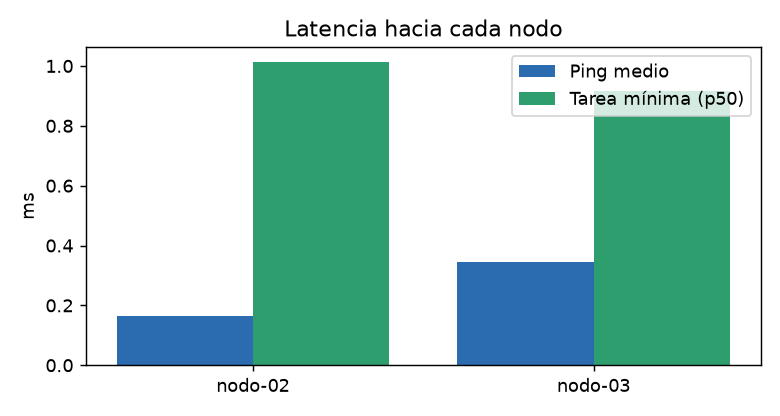
\includegraphics[width=0.7\textwidth]{figuras/latencia.png}
\caption{Latencia hacia cada nodo.}
\label{fig:latencia}
\end{figure}

\subsubsection{Tiempo de descubrimiento}

Se arranca un nodo nuevo, sin conocer a nadie, y se mide el tiempo hasta que descubre a todos los demás.

\begin{table}[htbp]
\centering
\small
\resizebox{\ifdim\width>\linewidth\linewidth\else\width\fi}{!}{%
\begin{tabular}{|c|c|c|c|}
\hline
\textbf{Intento} & \textbf{Segundos} & \textbf{Vecinos encontrados} & \textbf{Completo} \\ \hline
1 & 30.034 & 2 & no \\ \hline
2 & 30.038 & 2 & no \\ \hline
3 & 30.043 & 2 & no \\ \hline
4 & 0.203 & 3 & sí \\ \hline
5 & 0.102 & 3 & sí \\ \hline
6 & 0.101 & 3 & sí \\ \hline
7 & 0.102 & 3 & sí \\ \hline
8 & 0.101 & 3 & sí \\ \hline
\end{tabular}}
\caption{Tiempo de descubrimiento de un nodo nuevo.}
\label{tab:descubrimiento}
\end{table}

Descubrimiento completo en 5/8 intentos. En los 5 intentos completos tardó \textbf{0.12 s} de media (mín 0.10 s, máx 0.20 s). En los 3 restantes se agotó el límite de 30 s sin encontrar a todos los vecinos: el \emph{broadcast} UDP no tiene garantía de entrega y en una red Wi-Fi puede perderse; por eso el sistema también admite vecinos semilla por IP (\texttt{--peers}).

\subsubsection{Escalabilidad}

\paragraph{Más nodos, misma carga.} Se ejecuta el mismo lote de 24 tareas restringiendo el número de nodos disponibles.

\begin{table}[htbp]
\centering
\small
\resizebox{\ifdim\width>\linewidth\linewidth\else\width\fi}{!}{%
\begin{tabular}{|c|c|c|c|c|}
\hline
\textbf{Nodos} & \textbf{Tiempo total (s)} & \textbf{$\pm$ $\sigma$} & \textbf{Tareas/s} & \textbf{Aceleración} \\ \hline
1 & 2.621 & 0.26 & 9.26 & 1.0$\times$ \\ \hline
2 & 1.767 & 0.374 & 14.33 & 1.48$\times$ \\ \hline
3 & 1.69 & 0.137 & 14.29 & 1.55$\times$ \\ \hline
\end{tabular}}
\caption{Escalabilidad al aumentar el número de nodos.}
\label{tab:escal-nodos}
\end{table}

\begin{figure}[htbp]
\centering
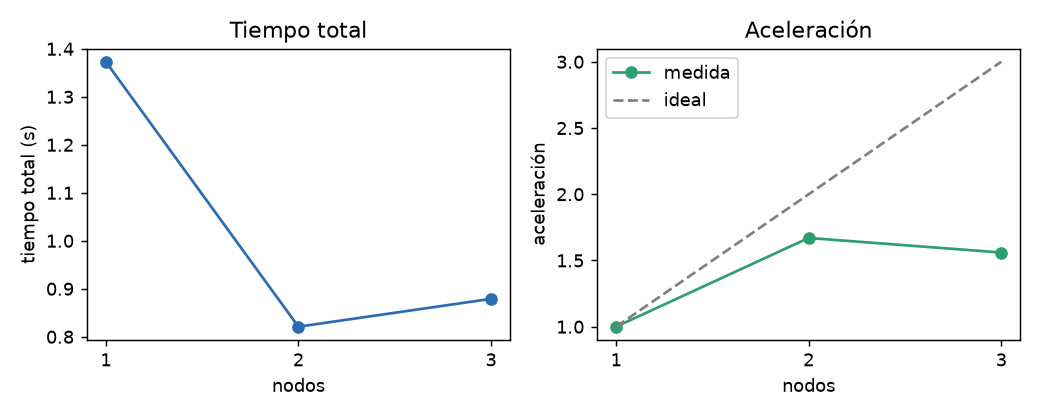
\includegraphics[width=0.9\textwidth]{figuras/escalabilidad_nodos.png}
\caption{Tiempo total y aceleración según el número de nodos.}
\label{fig:escal-nodos}
\end{figure}

Con 3 nodos la aceleración fue \textbf{1.55$\times$} (ideal: 3$\times$). La diferencia con el ideal se debe a la sobrecarga de coordinación (mensajes, ACK), a que las tareas se reparten en bloques discretos y a las diferencias de capacidad entre equipos.

\paragraph{Incremento progresivo de la carga.}

\begin{table}[htbp]
\centering
\small
\resizebox{\ifdim\width>\linewidth\linewidth\else\width\fi}{!}{%
\begin{tabular}{|c|c|c|c|c|c|c|}
\hline
\textbf{Tareas} & \textbf{Tiempo total (s)} & \textbf{Tareas/s} & \textbf{Latencia media (s)} & \textbf{p95 (s)} & \textbf{Tráfico enviado (KB/s)} & \textbf{CPU usada media (\%)} \\ \hline
4 & 0.222 & 17.99 & 0.197 & 0.221 & 6.79 & nodo-01: 24.5, nodo-03: 77.0, nodo-02: 20.2 \\ \hline
8 & 0.454 & 17.61 & 0.286 & 0.453 & 3.92 & nodo-01: 15.7, nodo-03: 77.0, nodo-02: 17.4 \\ \hline
16 & 1.291 & 12.4 & 0.487 & 0.898 & 2.71 & nodo-01: 21.1, nodo-03: 41.8, nodo-02: 17.4 \\ \hline
32 & 2.328 & 13.75 & 1.142 & 2.233 & 4.87 & nodo-01: 14.0, nodo-03: 52.6, nodo-02: 22.4 \\ \hline
64 & 4.417 & 14.49 & 1.455 & 3.801 & 3.57 & nodo-01: 17.3, nodo-03: 28.1, nodo-02: 23.4 \\ \hline
\end{tabular}}
\caption{Respuesta del sistema al aumentar la carga.}
\label{tab:escal-carga}
\end{table}

\begin{figure}[htbp]
\centering
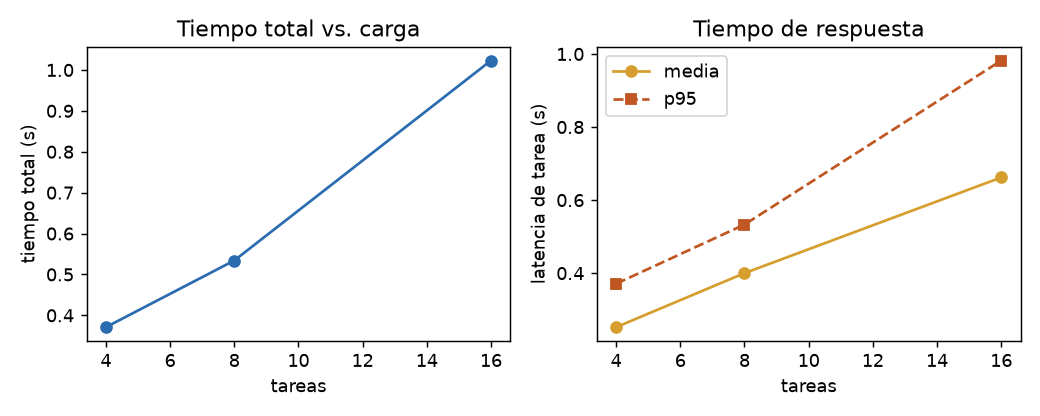
\includegraphics[width=0.9\textwidth]{figuras/carga_progresiva.png}
\caption{Tiempo total y tiempo de respuesta según la carga.}
\label{fig:escal-carga}
\end{figure}

Al multiplicar la carga por 16 (de 4 a 64 tareas) el tiempo total se multiplicó por 19.9 y el rendimiento pasó de 17.99 a 14.49 tareas/s. El tráfico de control fue de 3.57 KB/s con la mayor carga.

\subsubsection{Comparación de estrategias de asignación}

Mismo lote de 36 tareas de tamaño heterogéneo (0.5$\times$, 1$\times$ y 2$\times$) con cada estrategia. \emph{Desbalance} es el coeficiente de variación del número de tareas por nodo (0 = reparto perfecto).

\begin{table}[htbp]
\centering
\small
\resizebox{\ifdim\width>\linewidth\linewidth\else\width\fi}{!}{%
\begin{tabular}{|c|c|c|c|c|c|c|}
\hline
\textbf{Estrategia} & \textbf{Tiempo total (s)} & \textbf{$\pm$ $\sigma$} & \textbf{Latencia media (s)} & \textbf{p95 (s)} & \textbf{Desbalance} & \textbf{Tareas por nodo} \\ \hline
$F(i,j)$ del diseño & 5.029 & 2.334 & 2.621 & 4.929 & 1.414 & nodo-01: 0.0, nodo-02: 24.0, nodo-03: 12.0 \\ \hline
$F(i,j)$ + carga & 3.02 & 0.79 & 1.328 & 2.733 & 0.972 & nodo-01: 9.7, nodo-02: 20.7, nodo-03: 5.7 \\ \hline
Menos cargado & 2.948 & 0.408 & 0.944 & 2.603 & 0.0 & nodo-01: 12.0, nodo-02: 12.0, nodo-03: 12.0 \\ \hline
Menor latencia & 3.365 & 0.087 & 1.701 & 3.275 & 1.414 & nodo-01: 36.0, nodo-02: 0.0, nodo-03: 0.0 \\ \hline
Round-robin & 2.983 & 0.126 & 0.99 & 2.812 & 0.0 & nodo-01: 12.0, nodo-02: 12.0, nodo-03: 12.0 \\ \hline
Aleatoria & 3.078 & 0.34 & 1.011 & 2.855 & 0.203 & nodo-01: 9.7, nodo-02: 12.3, nodo-03: 14.0 \\ \hline
\end{tabular}}
\caption{Comparación de las seis estrategias de asignación.}
\label{tab:estrategias}
\end{table}

\begin{figure}[htbp]
\centering
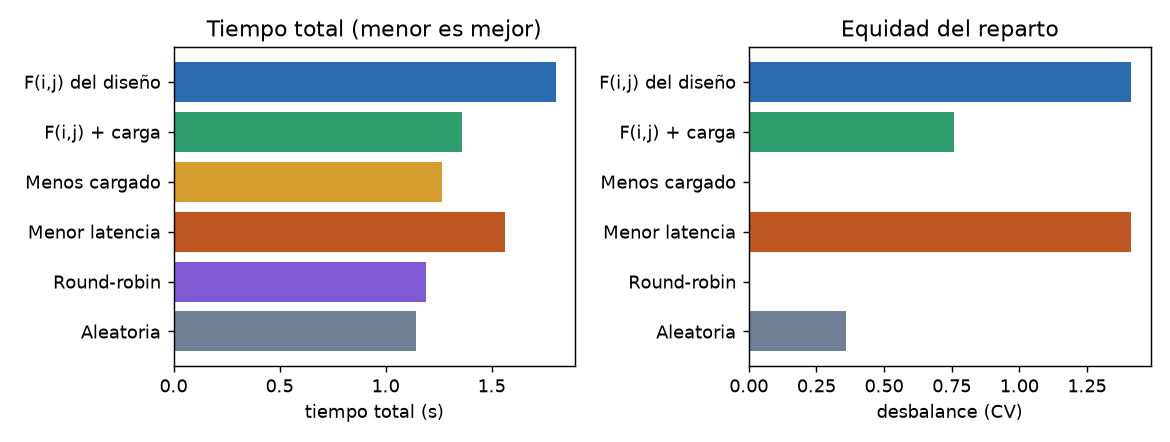
\includegraphics[width=0.9\textwidth]{figuras/estrategias.png}
\caption{Tiempo total y equidad del reparto por estrategia.}
\label{fig:estrategias}
\end{figure}

La estrategia con menor tiempo total fue \textbf{Menos cargado} (2.948 s) y la de mayor tiempo \textbf{$F(i,j)$ del diseño} (5.029 s). La función $F(i,j)$ del diseño original tardó 5.029 s con un desbalance de 1.414. Esa función no considera la carga actual y la normalización min-max convierte diferencias mínimas de CPU y memoria entre nodos desocupados en diferencias de 0 a 1, por lo que puede concentrar tareas en pocos nodos. La variante \texttt{weighted\_load} (término de carga y normalización robusta) redujo el tiempo total en 40\,\% y el desbalance de 1.414 a 0.972, conservando el criterio multicriterio.

\subsubsection{Tolerancia a fallos}

Un nodo cae 2 s después de empezar un lote de tareas (deja de enviar y recibir durante 25 s).

\begin{table}[htbp]
\centering
\small
\resizebox{\ifdim\width>\linewidth\linewidth\else\width\fi}{!}{%
\begin{tabular}{|c|c|c|c|c|c|c|c|c|}
\hline
\textbf{Intento} & \textbf{Nodo caído} & \textbf{Tareas} & \textbf{Completadas} & \textbf{\% completado} & \textbf{Reasignadas} & \textbf{Detección (s)} & \textbf{Recuperación (s)} & \textbf{Tiempo total (s)} \\ \hline
1 & nodo-02 & 20 & 20 & 100.0 & 10 & 4.25 & 4.16 & 10.41 \\ \hline
2 & nodo-03 & 20 & 20 & 100.0 & 4 & 5.38 & 1.22 & 8.61 \\ \hline
3 & nodo-02 & 20 & 20 & 100.0 & 15 & 4.31 & 6.06 & 12.38 \\ \hline
4 & nodo-03 & 20 & 20 & 100.0 & 4 & 4.98 & 1.18 & 8.17 \\ \hline
\end{tabular}}
\caption{Caída de un nodo durante la ejecución de un lote.}
\label{tab:fallos}
\end{table}

\begin{itemize}
\item Detección de la caída: media \textbf{4.73 s} (requisito: $\leq$ 5 s de silencio; la detección corre cada 0.5 s).
\item Tareas completadas pese a la caída: \textbf{100\,\%} (sin intervención manual).
\item La \emph{recuperación} es el tiempo desde la primera reasignación hasta que la tarea reasignada termina (incluye volver a ejecutarla).
\end{itemize}

\begin{figure}[htbp]
\centering
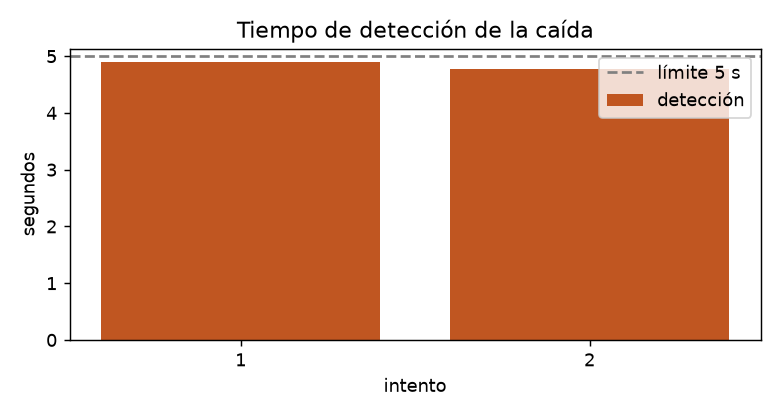
\includegraphics[width=0.7\textwidth]{figuras/tolerancia_fallos.png}
\caption{Tiempo de detección de la caída en cada intento.}
\label{fig:fallos}
\end{figure}

\subsubsection{Disponibilidad del servicio}

Cada 0.5 s se envía una tarea de sondeo mientras nodo-02 falla entre $t = 15$ s y $t = 35$ s.

\begin{table}[htbp]
\centering
\small
\resizebox{\ifdim\width>\linewidth\linewidth\else\width\fi}{!}{%
\begin{tabular}{|c|c|}
\hline
\textbf{Métrica} & \textbf{Valor} \\ \hline
Sondas enviadas & 140 \\ \hline
Completadas & 100.0 \% \\ \hline
Completadas en $\leq$ 3 s & 97.86 \% \\ \hline
\end{tabular}}
\caption{Disponibilidad del servicio durante la falla de un nodo.}
\label{tab:disponibilidad}
\end{table}

\begin{figure}[htbp]
\centering
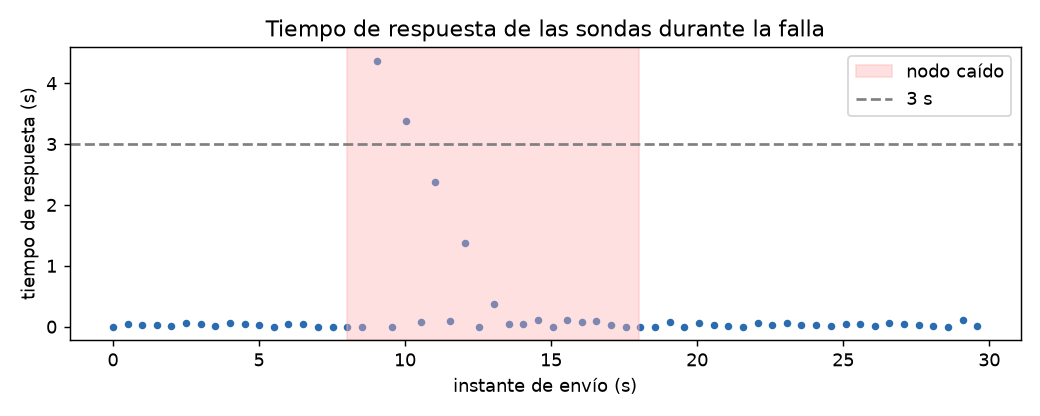
\includegraphics[width=0.9\textwidth]{figuras/disponibilidad.png}
\caption{Tiempo de respuesta de las sondas durante la falla.}
\label{fig:disponibilidad}
\end{figure}

Las sondas enviadas al nodo caído no reciben \texttt{TASK\_ACK}; tras el \emph{timeout} se reasignan a otro nodo y se completan, por eso la disponibilidad es alta pero algunas respuestas tardan alrededor del \emph{timeout} de 5 s.

\subsubsection{Consumo de recursos del nodo coordinador}

\begin{table}[htbp]
\centering
\small
\resizebox{\ifdim\width>\linewidth\linewidth\else\width\fi}{!}{%
\begin{tabular}{|c|c|}
\hline
\textbf{Métrica} & \textbf{Valor} \\ \hline
Mensajes enviados / recibidos & 2124 / 3469 \\ \hline
Tráfico enviado / recibido & 546 KB / 838 KB \\ \hline
Duración & 468 s \\ \hline
Tráfico medio enviado & 1.17 KB/s \\ \hline
Tareas enviadas / completadas / reasignadas / fallidas & 1308 / 1308 / 39 / 0 \\ \hline
\end{tabular}}
\caption{Consumo del nodo que coordinó los experimentos.}
\label{tab:recursos}
\end{table}

\subsubsection{Síntesis de los resultados}

\begin{itemize}
\item \textbf{Descubrimiento:} los nodos se encuentran solos en 0.12 s de media en 5/8 intentos, sin configuración manual.
\item \textbf{Escalabilidad:} con 3 nodos la aceleración fue 1.55$\times$ respecto a un solo nodo.
\item \textbf{Estrategias:} la de menor tiempo total fue Menos cargado.
\item \textbf{Fallos:} la caída se detectó en 4.73 s de media y se completó el 100\,\% de las tareas.
\item \textbf{Disponibilidad:} se completó el 100.0\,\% de las sondas durante la falla de un nodo.
\end{itemize}


\subsection{Pruebas}

El proyecto incluye 66 pruebas automáticas (\texttt{python -m pytest tests}): 42 de las fases anteriores
(planificador, mensajes, reloj de Lamport, tabla de vecinos, detector de fallos y escenarios de
integración con tres nodos reales) y 24 de la Fase 3, que verifican:

\begin{itemize}
\item las seis estrategias y su respeto por los requisitos de la tarea;
\item la normalización robusta (sin amplificar diferencias mínimas) y el ejemplo numérico del diseño;
\item que la suma de los estadísticos de los fragmentos equivale a la regresión sobre todos los datos;
\item la API (\texttt{map} conserva el orden, el requisito de nodos, el cambio de estrategia, \texttt{on\_event});
\item que una alerta llega al registro de todos los nodos;
\item que un nodo caído pasa a \texttt{OFFLINE}, se recupera y que sus tareas se reasignan;
\item que las ranuras limitan la ejecución simultánea y la detección de la subred.
\end{itemize}

\subsection{Qué se puede demostrar en la sustentación}

\begin{itemize}
\item Tres computadores físicos descubriéndose automáticamente en la misma red.
\item El panel web mostrando los tres nodos, sus recursos, la latencia y las tareas en vivo.
\item Las tres aplicaciones: alertas de monitoreo, procesamiento \emph{map-reduce} y regresión
lineal distribuida.
\item La caída de un nodo durante una tarea: alerta crítica, reasignación automática y resultado
correcto.
\item El cambio de estrategia de asignación en caliente y su efecto en el reparto.
\item Las métricas y gráficas de los experimentos.
\end{itemize}

\subsection{Limitaciones}

\begin{itemize}
\item El ancho de banda de cada nodo es un valor declarado, no medido.
\item UDP no garantiza la entrega ni hay retransmisión: la pérdida de un mensaje se maneja con el
\emph{timeout} de la confirmación y la reasignación de la tarea.
\item El nodo que envía una tarea la coordina; si ese nodo cae, pierde el estado de sus tareas, porque
no hay persistencia.
\item La sincronización es un orden lógico de eventos (Lamport); no hay exclusión mutua distribuida.
\item Los \emph{endpoints} de administración no tienen autenticación (uso de laboratorio).
\item Las tareas deben ser lo bastante grandes para amortizar el costo de la comunicación.
\end{itemize}

\subsection{Conclusión de la fase}

Con esta fase se completa ComplexNet API: una red de tres computadores físicos que se descubren solos,
reparten el trabajo con reglas locales, ejecutan aplicaciones de monitoreo, procesamiento y
aprendizaje automático distribuido, detectan fallos y se recuperan sin intervención humana ni
coordinador central. La API permite a otros desarrolladores crear nuevas aplicaciones con pocas líneas,
y la evaluación experimental respalda el comportamiento del sistema en latencia, escalabilidad,
disponibilidad y tolerancia a fallos. Del análisis de las estrategias de asignación resultó una mejora
al modelo original (normalización robusta y término de carga) que evita concentrar las tareas en un
solo nodo.

% Requiere solo el paquete graphicx (ya usado en las secciones anteriores).
% Las tablas y figuras de resultados se generan con
%         python experiments/report.py
% en el archivo fase3_resultados.tex (se incluye al final de esta sección).
% =============================================================================

\section{Descripción del Proyecto -- Fase 3}

\subsection{Objetivo de la fase}

En la Fase 2 se construyó el núcleo de ComplexNet API y se validó con tres nodos en contenedores
Docker dentro de un mismo computador. La Fase 3 convierte ese núcleo en una plataforma utilizable:
se ejecuta sobre \textbf{tres computadores físicos} conectados por una red local, ofrece una
\textbf{API documentada para desarrolladores}, incluye \textbf{tres aplicaciones descentralizadas}
construidas sobre ella, un \textbf{panel de monitoreo} del clúster y una \textbf{evaluación
experimental} de latencia, escalabilidad, disponibilidad, tolerancia a fallos y estrategias de
asignación de tareas.

\subsection{Qué se agregó respecto a la Fase 2}

El núcleo (mensajes JSON sobre UDP, descubrimiento por \emph{beacons}, detección de fallos por
silencio, reasignación de tareas y reloj lógico de Lamport) se mantiene. Lo nuevo es lo siguiente:

\begin{table}[htbp]
\centering
\small
\begin{tabular}{|p{0.2\textwidth}|p{0.33\textwidth}|p{0.33\textwidth}|}
\hline
\textbf{Aspecto} & \textbf{Fase 2} & \textbf{Fase 3} \\ \hline
Despliegue & Tres contenedores Docker en un computador, red virtual & Tres computadores físicos en una red local real \\ \hline
Descubrimiento & \emph{Broadcast} a una subred fija de Docker & Detección automática de la subred y vecinos semilla por IP \\ \hline
Uso del sistema & Script de demostración & API para desarrolladores y manual \\ \hline
Aplicaciones & Una tarea de regresión lineal de ejemplo & Tres aplicaciones descentralizadas \\ \hline
Monitoreo & Terminal y un archivo JSON por nodo & Panel web en vivo con alertas \\ \hline
Planificación & Una función de aptitud $F(i,j)$ & Seis estrategias intercambiables en caliente \\ \hline
Capacidad del nodo & Sin límite de tareas simultáneas & Ranuras de ejecución (\emph{slots}) y cola \\ \hline
Validación & Pruebas funcionales (42) & Pruebas (66) y experimentos con informe \\ \hline
\end{tabular}
\caption{Cambios de la Fase 3 respecto a la Fase 2.}
\label{tab:fase2-fase3}
\end{table}

\subsection{Despliegue en tres computadores}

\paragraph{¿Cómo se conectan los computadores?}
Los tres equipos se conectan a la \textbf{misma red local} (mismo Wi-Fi o router; también sirve el
punto de acceso de un celular). No se usa ningún servidor central ni se necesita internet: cada
nodo envía los mensajes directamente a los demás mediante \textbf{UDP sobre IP}, por el puerto
\texttt{9999}. El panel web usa el puerto \texttt{8000} (TCP) y es solo para observar y administrar.

\begin{table}[htbp]
\centering
\small
\begin{tabular}{|c|c|p{0.5\textwidth}|}
\hline
\textbf{Equipo} & \textbf{Nodo} & \textbf{Qué ejecuta} \\ \hline
Computador 1 & \texttt{nodo-01} & Un nodo, las aplicaciones y los experimentos \\ \hline
Computador 2 & \texttt{nodo-02} & Solo el nodo \\ \hline
Computador 3 & \texttt{nodo-03} & Solo el nodo \\ \hline
\end{tabular}
\caption{Distribución de nodos en los computadores.}
\label{tab:tres-pcs}
\end{table}

\paragraph{Descubrimiento en la red real.}
\begin{enumerate}
\item Cada nodo emite cada 2 s un mensaje \texttt{RESOURCE\_BEACON} por \emph{broadcast} UDP, es decir,
a la dirección que reciben todos los equipos de la subred. El nodo calcula esa dirección a partir de
su propia IP y máscara de red (opción \texttt{--broadcast auto}).
\item El \emph{beacon} informa el identificador del nodo, su IP, su CPU libre, su memoria libre, su ancho
de banda y cuántas tareas tiene en curso.
\item Al recibir el \emph{beacon} de un nodo desconocido, el receptor lo registra en su \texttt{PeerTable}
y le responde con un \emph{beacon} directo. Así, basta con que uno de los dos oiga al otro para que
ambos se descubran.
\item Si la red bloquea el \emph{broadcast} (algunas redes institucionales lo filtran), cada nodo puede
iniciarse con las IP de sus vecinos (\texttt{--peers}) y los mensajes viajan de forma directa. Otra
alternativa es conectar los tres equipos al punto de acceso de un celular.
\end{enumerate}

\paragraph{Mensajes del protocolo.}
Todos los mensajes son JSON con un encabezado (identificador único, emisor, tipo, marca de tiempo y
reloj de Lamport) y una carga útil. El tamaño máximo es de 60 KB, de modo que cada mensaje cabe en un
datagrama UDP.

\begin{table}[htbp]
\centering
\small
\begin{tabular}{|l|p{0.55\textwidth}|}
\hline
\textbf{Mensaje} & \textbf{Función} \\ \hline
\texttt{RESOURCE\_BEACON} & Presencia y recursos del nodo (cada 2 s) \\ \hline
\texttt{PING} / \texttt{PONG} & Medición de la latencia (RTT) entre dos nodos \\ \hline
\texttt{TASK\_SUBMIT} & Envío de una tarea al nodo elegido \\ \hline
\texttt{TASK\_ACK} & Confirmación de recepción de la tarea \\ \hline
\texttt{TASK\_RESULT} & Resultado de la tarea o error \\ \hline
\texttt{ALERT} & Alerta difundida a todos los nodos (Fase 3) \\ \hline
\end{tabular}
\caption{Mensajes intercambiados entre los nodos.}
\label{tab:mensajes}
\end{table}

\paragraph{Puesta en marcha.}
Cada computador ejecuta un único comando, que crea el entorno de Python, instala las dependencias,
abre el puerto en el cortafuegos y arranca el nodo:

\begin{verbatim}
.\scripts\start_node.ps1 -Id nodo-02
\end{verbatim}

\subsection{API para desarrolladores}

La clase \texttt{Node} es la puerta de entrada: oculta el descubrimiento, la planificación, la
comunicación y la recuperación ante fallos. Una aplicación necesita pocas líneas:

\begin{verbatim}
from complexnet import Node, Task

with Node("nodo-01", broadcast_address="auto") as node:
    node.wait_for_peers(2)
    tarea = Task("regresion_lineal", {"n_samples": 10000},
                 requirements={"cpu": 1, "memory": 256})
    resultado = node.submit(tarea)      # el planificador elige el nodo
\end{verbatim}

\begin{table}[htbp]
\centering
\small
\begin{tabular}{|p{0.3\textwidth}|p{0.6\textwidth}|}
\hline
\textbf{Método} & \textbf{Descripción} \\ \hline
\texttt{connect()}, \texttt{disconnect()} & Une el nodo a la red o lo detiene (también como \texttt{with}) \\ \hline
\texttt{wait\_for\_peers(n)} & Espera hasta tener $n$ vecinos activos \\ \hline
\texttt{submit(tarea)} & Envía una tarea y devuelve su resultado (o la tarea, sin esperar) \\ \hline
\texttt{map(nombre, lista)} & Una tarea por elemento; devuelve los resultados en orden \\ \hline
\texttt{map\_tasks(...)} & Igual que \texttt{map}, pero devuelve las tareas con sus tiempos y el nodo ejecutor \\ \hline
\texttt{broadcast(tipo, datos)} & Envía un mensaje a todos los vecinos activos \\ \hline
\texttt{raise\_alert(nivel, texto)} & Registra una alerta y la difunde a toda la red \\ \hline
\texttt{on\_event(funcion)} & Ejecuta una función por cada evento del nodo (fallos, tareas, descubrimiento) \\ \hline
\texttt{set\_strategy(nombre)} & Cambia la estrategia de asignación en caliente \\ \hline
\texttt{simulate\_failure(s)} & Simula una caída del nodo durante $s$ segundos (pruebas) \\ \hline
\texttt{status()} & Estado completo: recursos, vecinos, tareas, alertas y métricas \\ \hline
\end{tabular}
\caption{Métodos principales de la API.}
\label{tab:api}
\end{table}

Una \texttt{Task} lleva un nombre, sus parámetros y requisitos (CPU libre mínima, memoria mínima y,
opcionalmente, una lista de nodos permitidos). Los tipos de tarea disponibles son los siguientes:

\begin{table}[htbp]
\centering
\small
\begin{tabular}{|l|p{0.55\textwidth}|}
\hline
\textbf{Tarea} & \textbf{Descripción} \\ \hline
\texttt{regresion\_lineal} & Regresión lineal completa en un nodo (Fase 2) \\ \hline
\texttt{normal\_equations} & Estadísticos de un fragmento de datos para la regresión distribuida \\ \hline
\texttt{evaluate\_model} & Evaluación de un modelo sobre un fragmento de datos \\ \hline
\texttt{monte\_carlo\_pi} & Estimación de $\pi$ por el método de Monte Carlo \\ \hline
\texttt{word\_count} & Conteo de palabras de un fragmento de texto \\ \hline
\end{tabular}
\caption{Tipos de tarea incluidos.}
\label{tab:tareas}
\end{table}

Agregar una tarea nueva consiste en escribir una función de Python que reciba un diccionario y
devuelva otro, y registrarla en el módulo de ejecutores. La referencia completa está en el manual del
desarrollador (\texttt{docs/api/MANUAL\_DESARROLLADOR.md}).

\subsection{Aplicaciones descentralizadas}

Las tres aplicaciones usan únicamente la API anterior; ninguna depende de un servidor central.

\subsubsection{Aplicación 1: monitoreo distribuido con alertas}

Vigila el clúster con la información que ya circula en los \emph{beacons} y genera alertas que se
\textbf{difunden a todos los nodos}, de modo que cada nodo conserva su propio registro de alertas.

\begin{itemize}
\item \textbf{Crítica:} un nodo pasa a \texttt{OFFLINE}.
\item \textbf{Informativa:} un nodo vuelve a estar \texttt{ONLINE}.
\item \textbf{Advertencia:} CPU libre menor a un umbral, memoria libre menor a un umbral o latencia
mayor a un umbral (configurables).
\end{itemize}

Además guarda una serie de tiempo con la CPU, la memoria y la latencia de cada nodo, y las alertas
aparecen en el panel web.

\subsubsection{Aplicación 2: procesamiento distribuido}

Realiza dos trabajos de tipo \emph{map-reduce} repartidos por la red:

\begin{enumerate}
\item \textbf{Análisis de archivos:} los archivos de texto de una carpeta se parten en fragmentos; cada
nodo cuenta las palabras de su fragmento (\emph{map}) y el nodo coordinador combina los conteos
(\emph{reduce}).
\item \textbf{Cálculo colaborativo:} estimación de $\pi$ por Monte Carlo. Cada nodo lanza puntos al azar
en el cuadrado unidad y cuenta los que caen dentro del círculo; con el total se obtiene
$\pi \approx 4 \cdot \mathrm{dentro} / \mathrm{total}$.
\end{enumerate}

Si un nodo cae durante el trabajo, sus fragmentos se reasignan y el resultado no cambia.

\subsubsection{Aplicación 3: inteligencia artificial distribuida}

Entrena una \textbf{regresión lineal múltiple} repartiendo los datos entre los nodos. La idea es que
la solución de mínimos cuadrados se puede calcular a partir de sumas parciales. Si el conjunto de
datos se divide en fragmentos $(X_k, y_k)$, cada nodo calcula $X_k^{\top}X_k$ y $X_k^{\top}y_k$ de su
fragmento y el coordinador los suma y resuelve:

\begin{equation}
\hat{w} = \Bigl(\sum_k X_k^{\top}X_k\Bigr)^{-1} \sum_k X_k^{\top}y_k
\end{equation}

El resultado es exactamente el de entrenar con todos los datos en un solo equipo. Cada fragmento se
genera dentro del nodo que lo procesa a partir de una semilla, por lo que por la red solo viajan
parámetros pequeños y estadísticos. El modelo se evalúa después en fragmentos nuevos, también
repartidos, calculando el coeficiente de determinación
$R^2 = 1 - \mathrm{SSE}/\mathrm{SST}$. Si un nodo falla durante el entrenamiento, su fragmento se
reasigna a otro y los pesos finales son los mismos.

\begin{table}[htbp]
\centering
\small
\begin{tabular}{|p{0.28\textwidth}|p{0.62\textwidth}|}
\hline
\textbf{Requisito del taller} & \textbf{Cómo se cumple} \\ \hline
Distribución de datos & Fragmentos generados en cada nodo a partir de una semilla \\ \hline
Asignación de recursos & El planificador reparte cada fragmento según CPU, memoria, ancho de banda, latencia, reputación y carga \\ \hline
Información intercambiada & Estadísticos $X_k^{\top}X_k$, $X_k^{\top}y_k$ y sumas de cuadrados, no los datos \\ \hline
Métricas & Error de los pesos, $R^2$, MSE, tiempos y fragmentos por nodo \\ \hline
Tolerancia a fallos & Reasignación automática del fragmento del nodo caído \\ \hline
\end{tabular}
\caption{Aplicación de inteligencia artificial: cumplimiento de los requisitos.}
\label{tab:ia}
\end{table}

\subsection{Estrategias de asignación de tareas}

El planificador de la Fase 2 implementa la función de aptitud del diseño (sección 9):

\begin{equation}
F(i,j) = 0.40\,C' + 0.40\,M' + 0.10\,B' + 0.05\,R - 0.05\,(1 - L')
\end{equation}

donde $C'$, $M'$, $B'$ y $L'$ son la CPU libre, la memoria libre, el ancho de banda y la latencia
(esta última con normalización inversa) normalizados entre los candidatos, y $R$ es la reputación del
nodo. Al probarla en los experimentos se observó un problema: la normalización min-max convierte
diferencias mínimas entre nodos casi idénticos (por ejemplo, 1\,\% de CPU) en diferencias de 0 a 1, y
la función no conoce cuántas tareas tiene ya cada nodo, así que podía enviar todas las tareas al mismo
nodo.

Para resolverlo se agregó la variante \texttt{weighted\_load}, que usa por defecto:

\begin{itemize}
\item \textbf{Normalización robusta:} $x' = (x - \min x) / \max(\max x - \min x,\ \delta)$, donde
$\delta$ es un rango mínimo significativo ($\delta_C = 20$ puntos de CPU libre, $\delta_M = \delta_B = 20\,\%$
del mayor valor y $\delta_L = 5$ ms). Las diferencias de ruido ya no se amplifican.
\item \textbf{Término de carga:} se resta $0.30\,Q'$, donde $Q'$ es el número de tareas en curso del
nodo (incluidas las que el propio coordinador le acaba de enviar) normalizado entre los candidatos; los
pesos de CPU y memoria bajan a 0.25 para que la suma siga siendo 1.
\end{itemize}

\begin{equation}
F_{L}(i,j) = 0.25\,C' + 0.25\,M' + 0.10\,B' + 0.05\,R - 0.05\,(1 - L') - 0.30\,Q'
\end{equation}

Además se implementaron cuatro estrategias de referencia para compararlas:

\begin{table}[htbp]
\centering
\small
\begin{tabular}{|l|p{0.6\textwidth}|}
\hline
\textbf{Estrategia} & \textbf{Criterio} \\ \hline
\texttt{weighted} & $F(i,j)$ del diseño \\ \hline
\texttt{weighted\_load} & $F_L(i,j)$: robusta y con carga (por defecto) \\ \hline
\texttt{least\_loaded} & El nodo con menos tareas en curso \\ \hline
\texttt{lowest\_latency} & El nodo con menor latencia medida \\ \hline
\texttt{round\_robin} & Reparto cíclico entre los candidatos aptos \\ \hline
\texttt{random} & Un candidato apto al azar \\ \hline
\end{tabular}
\caption{Estrategias de asignación implementadas.}
\label{tab:estrategias-lista}
\end{table}

En todas, el conjunto de candidatos se filtra primero con los requisitos de la tarea
($C_i \geq C_{\mathrm{req}}$ y $M_i \geq M_{\mathrm{req}}$) y solo se consideran los nodos activos.

\paragraph{Capacidad de los nodos.}
Cada nodo ejecuta como máximo \texttt{slots} tareas a la vez (2 por defecto); las demás esperan en cola.
Esto modela un computador con CPU limitada y hace que el reparto de carga sea relevante.

\subsection{Panel de monitoreo del clúster}

Cada nodo sirve una página web (\texttt{http://IP-DEL-NODO:8000}) que muestra, en tiempo real, los
nodos del clúster con su estado, CPU, memoria y latencia, la evolución de la latencia, las tareas y sus
resultados, las alertas y el registro de eventos. El mismo servicio expone una API HTTP: consulta del
estado (\texttt{GET /status}, \texttt{GET /events}), envío de tareas (\texttt{POST /tasks}) y
administración para los experimentos (\texttt{POST /admin/fail} para simular una caída remota y
\texttt{POST /admin/strategy} para cambiar la estrategia).

\subsection{Metodología experimental}

Los experimentos se ejecutan con \texttt{experiments/run\_experiments.py} desde el computador 1 y el
informe se genera con \texttt{experiments/report.py} a partir de los archivos CSV resultantes. La carga
de trabajo son tareas de Monte Carlo (intensivas en CPU), y cada medición se repite varias veces para
reportar la media y la desviación estándar. Se evalúan:

\begin{itemize}
\item \textbf{Latencia:} RTT de \texttt{PING}/\texttt{PONG} y tiempo de una tarea mínima.
\item \textbf{Tiempo de descubrimiento:} desde que arranca un nodo nuevo hasta conocer a los demás.
\item \textbf{Escalabilidad:} el mismo lote con 1, 2 y 3 nodos (aceleración) y cargas crecientes.
\item \textbf{Estrategias de asignación:} el mismo lote heterogéneo con las seis estrategias.
\item \textbf{Tolerancia a fallos:} un nodo cae a mitad de un lote y se mide la detección, la
recuperación y el porcentaje de tareas completadas.
\item \textbf{Disponibilidad:} se envía una tarea de sondeo cada 0.5 s mientras un nodo falla.
\end{itemize}

Las fallas se inyectan con el endpoint \texttt{/admin/fail} del nodo víctima, que deja de enviar y
recibir mensajes durante unos segundos, lo que equivale a una caída o a una desconexión de la red.

\subsection{Resultados experimentales}

Las tablas y gráficas de esta sección se generan automáticamente a partir de los datos medidos.

% ARCHIVO GENERADO por experiments/report.py -- no editar a mano.
% Corrida: 20261126-104206

\subsubsection{Entorno}

\begin{table}[htbp]
\centering
\small
\resizebox{\ifdim\width>\linewidth\linewidth\else\width\fi}{!}{%
\begin{tabular}{|c|c|}
\hline
\textbf{Dato} & \textbf{Valor} \\ \hline
Fecha & 2026-11-26 10:42:06 \\ \hline
Entorno & 3 computadores en red local \\ \hline
Nodos & nodo-01 (172.25.4.83), nodo-03 (172.25.5.66), nodo-02 (172.25.7.119) \\ \hline
Equipo que ejecutó los experimentos & MSI (Windows-11-10.0.26200-SP0) \\ \hline
CPU / RAM de ese equipo & 12 hilos / 15.7 GB \\ \hline
Python & 3.13.7 \\ \hline
Estrategia por defecto & weighted\_load \\ \hline
Tamaño de tarea (puntos Monte Carlo) & 12,000,000 \\ \hline
Modo & completo \\ \hline
\end{tabular}}
\caption{Entorno de la corrida experimental.}
\label{tab:entorno}
\end{table}

Los experimentos se ejecutaron en \textbf{tres computadores físicos} conectados a la misma red local, un nodo por computador.

\subsubsection{Latencia de comunicación}

\begin{table}[htbp]
\centering
\small
\resizebox{\ifdim\width>\linewidth\linewidth\else\width\fi}{!}{%
\begin{tabular}{|c|c|c|c|c|c|}
\hline
\textbf{Nodo} & \textbf{Ping medio (ms)} & \textbf{Ping mín (ms)} & \textbf{Ping máx (ms)} & \textbf{Tarea mínima p50 (ms)} & \textbf{Tarea mínima p95 (ms)} \\ \hline
nodo-02 & 61.116 & 30.221 & 136.877 & 7.733 & 26.384 \\ \hline
nodo-03 & 24.971 & 16.617 & 38.265 & 9.414 & 21.802 \\ \hline
\end{tabular}}
\caption{Latencia hacia cada nodo.}
\label{tab:latencia}
\end{table}

\emph{Ping} es el RTT de los mensajes \texttt{PING}/\texttt{PONG} que cada nodo mide a sus vecinos. \emph{Tarea mínima} es el tiempo completo de una tarea \texttt{echo} (asignación, envío, ejecución y respuesta).

\begin{figure}[htbp]
\centering
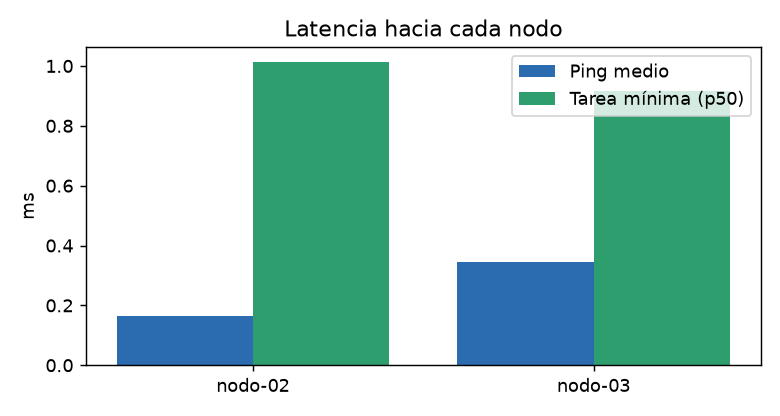
\includegraphics[width=0.7\textwidth]{figuras/latencia.png}
\caption{Latencia hacia cada nodo.}
\label{fig:latencia}
\end{figure}

\subsubsection{Tiempo de descubrimiento}

Se arranca un nodo nuevo, sin conocer a nadie, y se mide el tiempo hasta que descubre a todos los demás.

\begin{table}[htbp]
\centering
\small
\resizebox{\ifdim\width>\linewidth\linewidth\else\width\fi}{!}{%
\begin{tabular}{|c|c|c|c|}
\hline
\textbf{Intento} & \textbf{Segundos} & \textbf{Vecinos encontrados} & \textbf{Completo} \\ \hline
1 & 30.034 & 2 & no \\ \hline
2 & 30.038 & 2 & no \\ \hline
3 & 30.043 & 2 & no \\ \hline
4 & 0.203 & 3 & sí \\ \hline
5 & 0.102 & 3 & sí \\ \hline
6 & 0.101 & 3 & sí \\ \hline
7 & 0.102 & 3 & sí \\ \hline
8 & 0.101 & 3 & sí \\ \hline
\end{tabular}}
\caption{Tiempo de descubrimiento de un nodo nuevo.}
\label{tab:descubrimiento}
\end{table}

Descubrimiento completo en 5/8 intentos. En los 5 intentos completos tardó \textbf{0.12 s} de media (mín 0.10 s, máx 0.20 s). En los 3 restantes se agotó el límite de 30 s sin encontrar a todos los vecinos: el \emph{broadcast} UDP no tiene garantía de entrega y en una red Wi-Fi puede perderse; por eso el sistema también admite vecinos semilla por IP (\texttt{--peers}).

\subsubsection{Escalabilidad}

\paragraph{Más nodos, misma carga.} Se ejecuta el mismo lote de 24 tareas restringiendo el número de nodos disponibles.

\begin{table}[htbp]
\centering
\small
\resizebox{\ifdim\width>\linewidth\linewidth\else\width\fi}{!}{%
\begin{tabular}{|c|c|c|c|c|}
\hline
\textbf{Nodos} & \textbf{Tiempo total (s)} & \textbf{$\pm$ $\sigma$} & \textbf{Tareas/s} & \textbf{Aceleración} \\ \hline
1 & 2.621 & 0.26 & 9.26 & 1.0$\times$ \\ \hline
2 & 1.767 & 0.374 & 14.33 & 1.48$\times$ \\ \hline
3 & 1.69 & 0.137 & 14.29 & 1.55$\times$ \\ \hline
\end{tabular}}
\caption{Escalabilidad al aumentar el número de nodos.}
\label{tab:escal-nodos}
\end{table}

\begin{figure}[htbp]
\centering
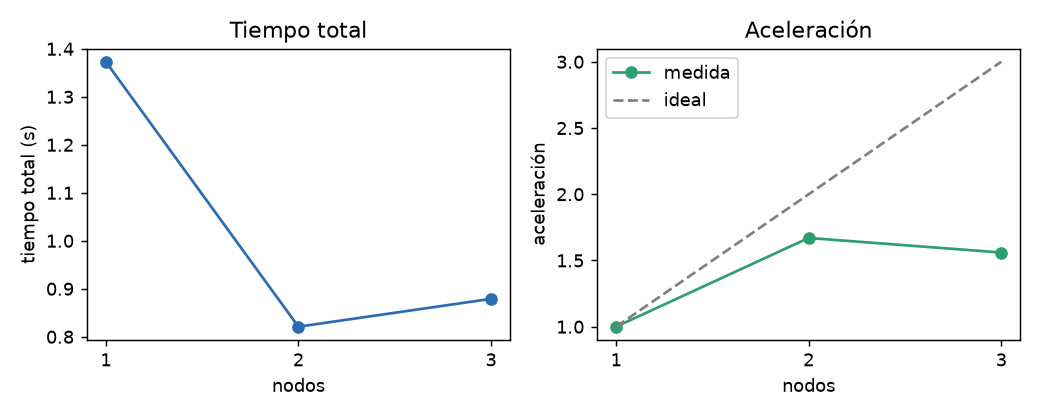
\includegraphics[width=0.9\textwidth]{figuras/escalabilidad_nodos.png}
\caption{Tiempo total y aceleración según el número de nodos.}
\label{fig:escal-nodos}
\end{figure}

Con 3 nodos la aceleración fue \textbf{1.55$\times$} (ideal: 3$\times$). La diferencia con el ideal se debe a la sobrecarga de coordinación (mensajes, ACK), a que las tareas se reparten en bloques discretos y a las diferencias de capacidad entre equipos.

\paragraph{Incremento progresivo de la carga.}

\begin{table}[htbp]
\centering
\small
\resizebox{\ifdim\width>\linewidth\linewidth\else\width\fi}{!}{%
\begin{tabular}{|c|c|c|c|c|c|c|}
\hline
\textbf{Tareas} & \textbf{Tiempo total (s)} & \textbf{Tareas/s} & \textbf{Latencia media (s)} & \textbf{p95 (s)} & \textbf{Tráfico enviado (KB/s)} & \textbf{CPU usada media (\%)} \\ \hline
4 & 0.222 & 17.99 & 0.197 & 0.221 & 6.79 & nodo-01: 24.5, nodo-03: 77.0, nodo-02: 20.2 \\ \hline
8 & 0.454 & 17.61 & 0.286 & 0.453 & 3.92 & nodo-01: 15.7, nodo-03: 77.0, nodo-02: 17.4 \\ \hline
16 & 1.291 & 12.4 & 0.487 & 0.898 & 2.71 & nodo-01: 21.1, nodo-03: 41.8, nodo-02: 17.4 \\ \hline
32 & 2.328 & 13.75 & 1.142 & 2.233 & 4.87 & nodo-01: 14.0, nodo-03: 52.6, nodo-02: 22.4 \\ \hline
64 & 4.417 & 14.49 & 1.455 & 3.801 & 3.57 & nodo-01: 17.3, nodo-03: 28.1, nodo-02: 23.4 \\ \hline
\end{tabular}}
\caption{Respuesta del sistema al aumentar la carga.}
\label{tab:escal-carga}
\end{table}

\begin{figure}[htbp]
\centering
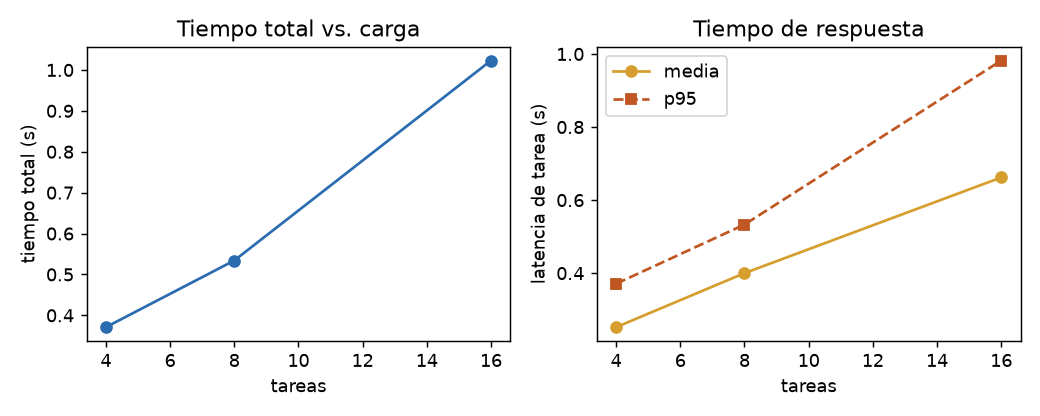
\includegraphics[width=0.9\textwidth]{figuras/carga_progresiva.png}
\caption{Tiempo total y tiempo de respuesta según la carga.}
\label{fig:escal-carga}
\end{figure}

Al multiplicar la carga por 16 (de 4 a 64 tareas) el tiempo total se multiplicó por 19.9 y el rendimiento pasó de 17.99 a 14.49 tareas/s. El tráfico de control fue de 3.57 KB/s con la mayor carga.

\subsubsection{Comparación de estrategias de asignación}

Mismo lote de 36 tareas de tamaño heterogéneo (0.5$\times$, 1$\times$ y 2$\times$) con cada estrategia. \emph{Desbalance} es el coeficiente de variación del número de tareas por nodo (0 = reparto perfecto).

\begin{table}[htbp]
\centering
\small
\resizebox{\ifdim\width>\linewidth\linewidth\else\width\fi}{!}{%
\begin{tabular}{|c|c|c|c|c|c|c|}
\hline
\textbf{Estrategia} & \textbf{Tiempo total (s)} & \textbf{$\pm$ $\sigma$} & \textbf{Latencia media (s)} & \textbf{p95 (s)} & \textbf{Desbalance} & \textbf{Tareas por nodo} \\ \hline
$F(i,j)$ del diseño & 5.029 & 2.334 & 2.621 & 4.929 & 1.414 & nodo-01: 0.0, nodo-02: 24.0, nodo-03: 12.0 \\ \hline
$F(i,j)$ + carga & 3.02 & 0.79 & 1.328 & 2.733 & 0.972 & nodo-01: 9.7, nodo-02: 20.7, nodo-03: 5.7 \\ \hline
Menos cargado & 2.948 & 0.408 & 0.944 & 2.603 & 0.0 & nodo-01: 12.0, nodo-02: 12.0, nodo-03: 12.0 \\ \hline
Menor latencia & 3.365 & 0.087 & 1.701 & 3.275 & 1.414 & nodo-01: 36.0, nodo-02: 0.0, nodo-03: 0.0 \\ \hline
Round-robin & 2.983 & 0.126 & 0.99 & 2.812 & 0.0 & nodo-01: 12.0, nodo-02: 12.0, nodo-03: 12.0 \\ \hline
Aleatoria & 3.078 & 0.34 & 1.011 & 2.855 & 0.203 & nodo-01: 9.7, nodo-02: 12.3, nodo-03: 14.0 \\ \hline
\end{tabular}}
\caption{Comparación de las seis estrategias de asignación.}
\label{tab:estrategias}
\end{table}

\begin{figure}[htbp]
\centering
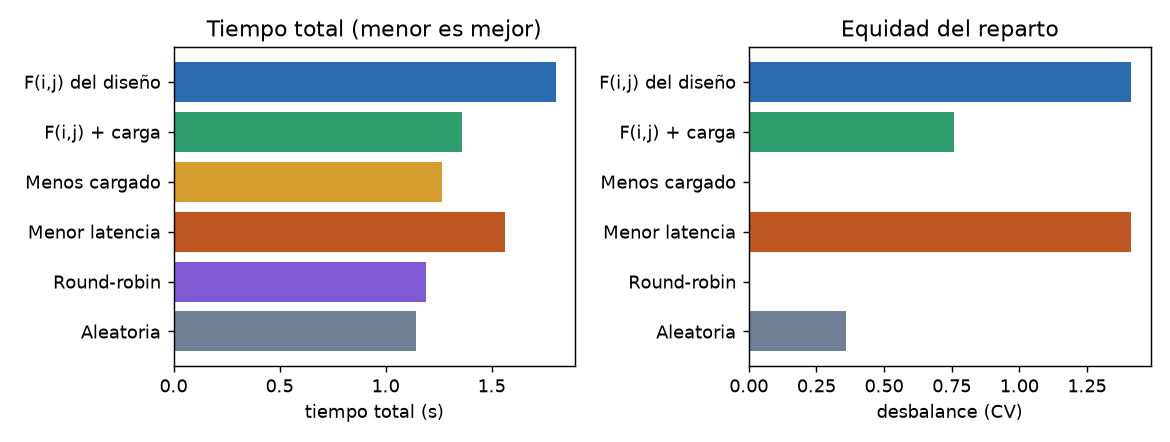
\includegraphics[width=0.9\textwidth]{figuras/estrategias.png}
\caption{Tiempo total y equidad del reparto por estrategia.}
\label{fig:estrategias}
\end{figure}

La estrategia con menor tiempo total fue \textbf{Menos cargado} (2.948 s) y la de mayor tiempo \textbf{$F(i,j)$ del diseño} (5.029 s). La función $F(i,j)$ del diseño original tardó 5.029 s con un desbalance de 1.414. Esa función no considera la carga actual y la normalización min-max convierte diferencias mínimas de CPU y memoria entre nodos desocupados en diferencias de 0 a 1, por lo que puede concentrar tareas en pocos nodos. La variante \texttt{weighted\_load} (término de carga y normalización robusta) redujo el tiempo total en 40\,\% y el desbalance de 1.414 a 0.972, conservando el criterio multicriterio.

\subsubsection{Tolerancia a fallos}

Un nodo cae 2 s después de empezar un lote de tareas (deja de enviar y recibir durante 25 s).

\begin{table}[htbp]
\centering
\small
\resizebox{\ifdim\width>\linewidth\linewidth\else\width\fi}{!}{%
\begin{tabular}{|c|c|c|c|c|c|c|c|c|}
\hline
\textbf{Intento} & \textbf{Nodo caído} & \textbf{Tareas} & \textbf{Completadas} & \textbf{\% completado} & \textbf{Reasignadas} & \textbf{Detección (s)} & \textbf{Recuperación (s)} & \textbf{Tiempo total (s)} \\ \hline
1 & nodo-02 & 20 & 20 & 100.0 & 10 & 4.25 & 4.16 & 10.41 \\ \hline
2 & nodo-03 & 20 & 20 & 100.0 & 4 & 5.38 & 1.22 & 8.61 \\ \hline
3 & nodo-02 & 20 & 20 & 100.0 & 15 & 4.31 & 6.06 & 12.38 \\ \hline
4 & nodo-03 & 20 & 20 & 100.0 & 4 & 4.98 & 1.18 & 8.17 \\ \hline
\end{tabular}}
\caption{Caída de un nodo durante la ejecución de un lote.}
\label{tab:fallos}
\end{table}

\begin{itemize}
\item Detección de la caída: media \textbf{4.73 s} (requisito: $\leq$ 5 s de silencio; la detección corre cada 0.5 s).
\item Tareas completadas pese a la caída: \textbf{100\,\%} (sin intervención manual).
\item La \emph{recuperación} es el tiempo desde la primera reasignación hasta que la tarea reasignada termina (incluye volver a ejecutarla).
\end{itemize}

\begin{figure}[htbp]
\centering
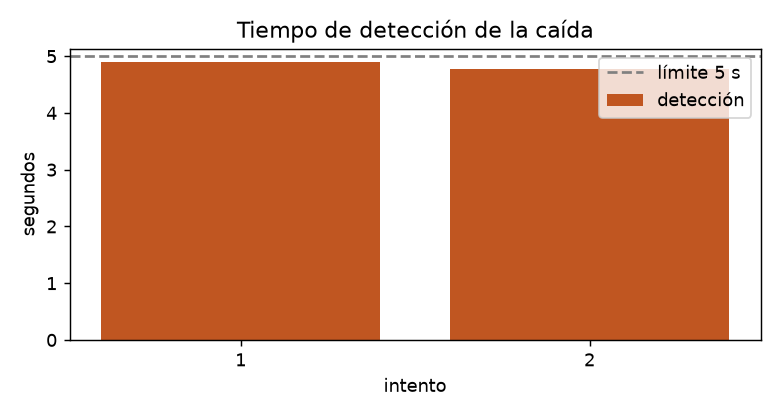
\includegraphics[width=0.7\textwidth]{figuras/tolerancia_fallos.png}
\caption{Tiempo de detección de la caída en cada intento.}
\label{fig:fallos}
\end{figure}

\subsubsection{Disponibilidad del servicio}

Cada 0.5 s se envía una tarea de sondeo mientras nodo-02 falla entre $t = 15$ s y $t = 35$ s.

\begin{table}[htbp]
\centering
\small
\resizebox{\ifdim\width>\linewidth\linewidth\else\width\fi}{!}{%
\begin{tabular}{|c|c|}
\hline
\textbf{Métrica} & \textbf{Valor} \\ \hline
Sondas enviadas & 140 \\ \hline
Completadas & 100.0 \% \\ \hline
Completadas en $\leq$ 3 s & 97.86 \% \\ \hline
\end{tabular}}
\caption{Disponibilidad del servicio durante la falla de un nodo.}
\label{tab:disponibilidad}
\end{table}

\begin{figure}[htbp]
\centering
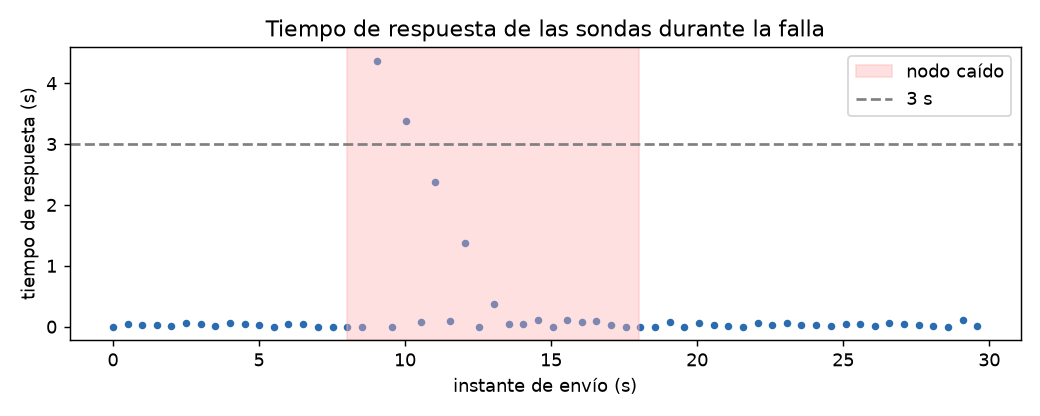
\includegraphics[width=0.9\textwidth]{figuras/disponibilidad.png}
\caption{Tiempo de respuesta de las sondas durante la falla.}
\label{fig:disponibilidad}
\end{figure}

Las sondas enviadas al nodo caído no reciben \texttt{TASK\_ACK}; tras el \emph{timeout} se reasignan a otro nodo y se completan, por eso la disponibilidad es alta pero algunas respuestas tardan alrededor del \emph{timeout} de 5 s.

\subsubsection{Consumo de recursos del nodo coordinador}

\begin{table}[htbp]
\centering
\small
\resizebox{\ifdim\width>\linewidth\linewidth\else\width\fi}{!}{%
\begin{tabular}{|c|c|}
\hline
\textbf{Métrica} & \textbf{Valor} \\ \hline
Mensajes enviados / recibidos & 2124 / 3469 \\ \hline
Tráfico enviado / recibido & 546 KB / 838 KB \\ \hline
Duración & 468 s \\ \hline
Tráfico medio enviado & 1.17 KB/s \\ \hline
Tareas enviadas / completadas / reasignadas / fallidas & 1308 / 1308 / 39 / 0 \\ \hline
\end{tabular}}
\caption{Consumo del nodo que coordinó los experimentos.}
\label{tab:recursos}
\end{table}

\subsubsection{Síntesis de los resultados}

\begin{itemize}
\item \textbf{Descubrimiento:} los nodos se encuentran solos en 0.12 s de media en 5/8 intentos, sin configuración manual.
\item \textbf{Escalabilidad:} con 3 nodos la aceleración fue 1.55$\times$ respecto a un solo nodo.
\item \textbf{Estrategias:} la de menor tiempo total fue Menos cargado.
\item \textbf{Fallos:} la caída se detectó en 4.73 s de media y se completó el 100\,\% de las tareas.
\item \textbf{Disponibilidad:} se completó el 100.0\,\% de las sondas durante la falla de un nodo.
\end{itemize}


\subsection{Pruebas}

El proyecto incluye 66 pruebas automáticas (\texttt{python -m pytest tests}): 42 de las fases anteriores
(planificador, mensajes, reloj de Lamport, tabla de vecinos, detector de fallos y escenarios de
integración con tres nodos reales) y 24 de la Fase 3, que verifican:

\begin{itemize}
\item las seis estrategias y su respeto por los requisitos de la tarea;
\item la normalización robusta (sin amplificar diferencias mínimas) y el ejemplo numérico del diseño;
\item que la suma de los estadísticos de los fragmentos equivale a la regresión sobre todos los datos;
\item la API (\texttt{map} conserva el orden, el requisito de nodos, el cambio de estrategia, \texttt{on\_event});
\item que una alerta llega al registro de todos los nodos;
\item que un nodo caído pasa a \texttt{OFFLINE}, se recupera y que sus tareas se reasignan;
\item que las ranuras limitan la ejecución simultánea y la detección de la subred.
\end{itemize}

\subsection{Qué se puede demostrar en la sustentación}

\begin{itemize}
\item Tres computadores físicos descubriéndose automáticamente en la misma red.
\item El panel web mostrando los tres nodos, sus recursos, la latencia y las tareas en vivo.
\item Las tres aplicaciones: alertas de monitoreo, procesamiento \emph{map-reduce} y regresión
lineal distribuida.
\item La caída de un nodo durante una tarea: alerta crítica, reasignación automática y resultado
correcto.
\item El cambio de estrategia de asignación en caliente y su efecto en el reparto.
\item Las métricas y gráficas de los experimentos.
\end{itemize}

\subsection{Limitaciones}

\begin{itemize}
\item El ancho de banda de cada nodo es un valor declarado, no medido.
\item UDP no garantiza la entrega ni hay retransmisión: la pérdida de un mensaje se maneja con el
\emph{timeout} de la confirmación y la reasignación de la tarea.
\item El nodo que envía una tarea la coordina; si ese nodo cae, pierde el estado de sus tareas, porque
no hay persistencia.
\item La sincronización es un orden lógico de eventos (Lamport); no hay exclusión mutua distribuida.
\item Los \emph{endpoints} de administración no tienen autenticación (uso de laboratorio).
\item Las tareas deben ser lo bastante grandes para amortizar el costo de la comunicación.
\end{itemize}

\subsection{Conclusión de la fase}

Con esta fase se completa ComplexNet API: una red de tres computadores físicos que se descubren solos,
reparten el trabajo con reglas locales, ejecutan aplicaciones de monitoreo, procesamiento y
aprendizaje automático distribuido, detectan fallos y se recuperan sin intervención humana ni
coordinador central. La API permite a otros desarrolladores crear nuevas aplicaciones con pocas líneas,
y la evaluación experimental respalda el comportamiento del sistema en latencia, escalabilidad,
disponibilidad y tolerancia a fallos. Del análisis de las estrategias de asignación resultó una mejora
al modelo original (normalización robusta y término de carga) que evita concentrar las tareas en un
solo nodo.

% Requiere solo el paquete graphicx (ya usado en las secciones anteriores).
% Las tablas y figuras de resultados se generan con
%         python experiments/report.py
% en el archivo fase3_resultados.tex (se incluye al final de esta sección).
% =============================================================================

\section{Descripción del Proyecto -- Fase 3}

\subsection{Objetivo de la fase}

En la Fase 2 se construyó el núcleo de ComplexNet API y se validó con tres nodos en contenedores
Docker dentro de un mismo computador. La Fase 3 convierte ese núcleo en una plataforma utilizable:
se ejecuta sobre \textbf{tres computadores físicos} conectados por una red local, ofrece una
\textbf{API documentada para desarrolladores}, incluye \textbf{tres aplicaciones descentralizadas}
construidas sobre ella, un \textbf{panel de monitoreo} del clúster y una \textbf{evaluación
experimental} de latencia, escalabilidad, disponibilidad, tolerancia a fallos y estrategias de
asignación de tareas.

\subsection{Qué se agregó respecto a la Fase 2}

El núcleo (mensajes JSON sobre UDP, descubrimiento por \emph{beacons}, detección de fallos por
silencio, reasignación de tareas y reloj lógico de Lamport) se mantiene. Lo nuevo es lo siguiente:

\begin{table}[htbp]
\centering
\small
\begin{tabular}{|p{0.2\textwidth}|p{0.33\textwidth}|p{0.33\textwidth}|}
\hline
\textbf{Aspecto} & \textbf{Fase 2} & \textbf{Fase 3} \\ \hline
Despliegue & Tres contenedores Docker en un computador, red virtual & Tres computadores físicos en una red local real \\ \hline
Descubrimiento & \emph{Broadcast} a una subred fija de Docker & Detección automática de la subred y vecinos semilla por IP \\ \hline
Uso del sistema & Script de demostración & API para desarrolladores y manual \\ \hline
Aplicaciones & Una tarea de regresión lineal de ejemplo & Tres aplicaciones descentralizadas \\ \hline
Monitoreo & Terminal y un archivo JSON por nodo & Panel web en vivo con alertas \\ \hline
Planificación & Una función de aptitud $F(i,j)$ & Seis estrategias intercambiables en caliente \\ \hline
Capacidad del nodo & Sin límite de tareas simultáneas & Ranuras de ejecución (\emph{slots}) y cola \\ \hline
Validación & Pruebas funcionales (42) & Pruebas (66) y experimentos con informe \\ \hline
\end{tabular}
\caption{Cambios de la Fase 3 respecto a la Fase 2.}
\label{tab:fase2-fase3}
\end{table}

\subsection{Despliegue en tres computadores}

\paragraph{¿Cómo se conectan los computadores?}
Los tres equipos se conectan a la \textbf{misma red local} (mismo Wi-Fi o router; también sirve el
punto de acceso de un celular). No se usa ningún servidor central ni se necesita internet: cada
nodo envía los mensajes directamente a los demás mediante \textbf{UDP sobre IP}, por el puerto
\texttt{9999}. El panel web usa el puerto \texttt{8000} (TCP) y es solo para observar y administrar.

\begin{table}[htbp]
\centering
\small
\begin{tabular}{|c|c|p{0.5\textwidth}|}
\hline
\textbf{Equipo} & \textbf{Nodo} & \textbf{Qué ejecuta} \\ \hline
Computador 1 & \texttt{nodo-01} & Un nodo, las aplicaciones y los experimentos \\ \hline
Computador 2 & \texttt{nodo-02} & Solo el nodo \\ \hline
Computador 3 & \texttt{nodo-03} & Solo el nodo \\ \hline
\end{tabular}
\caption{Distribución de nodos en los computadores.}
\label{tab:tres-pcs}
\end{table}

\paragraph{Descubrimiento en la red real.}
\begin{enumerate}
\item Cada nodo emite cada 2 s un mensaje \texttt{RESOURCE\_BEACON} por \emph{broadcast} UDP, es decir,
a la dirección que reciben todos los equipos de la subred. El nodo calcula esa dirección a partir de
su propia IP y máscara de red (opción \texttt{--broadcast auto}).
\item El \emph{beacon} informa el identificador del nodo, su IP, su CPU libre, su memoria libre, su ancho
de banda y cuántas tareas tiene en curso.
\item Al recibir el \emph{beacon} de un nodo desconocido, el receptor lo registra en su \texttt{PeerTable}
y le responde con un \emph{beacon} directo. Así, basta con que uno de los dos oiga al otro para que
ambos se descubran.
\item Si la red bloquea el \emph{broadcast} (algunas redes institucionales lo filtran), cada nodo puede
iniciarse con las IP de sus vecinos (\texttt{--peers}) y los mensajes viajan de forma directa. Otra
alternativa es conectar los tres equipos al punto de acceso de un celular.
\end{enumerate}

\paragraph{Mensajes del protocolo.}
Todos los mensajes son JSON con un encabezado (identificador único, emisor, tipo, marca de tiempo y
reloj de Lamport) y una carga útil. El tamaño máximo es de 60 KB, de modo que cada mensaje cabe en un
datagrama UDP.

\begin{table}[htbp]
\centering
\small
\begin{tabular}{|l|p{0.55\textwidth}|}
\hline
\textbf{Mensaje} & \textbf{Función} \\ \hline
\texttt{RESOURCE\_BEACON} & Presencia y recursos del nodo (cada 2 s) \\ \hline
\texttt{PING} / \texttt{PONG} & Medición de la latencia (RTT) entre dos nodos \\ \hline
\texttt{TASK\_SUBMIT} & Envío de una tarea al nodo elegido \\ \hline
\texttt{TASK\_ACK} & Confirmación de recepción de la tarea \\ \hline
\texttt{TASK\_RESULT} & Resultado de la tarea o error \\ \hline
\texttt{ALERT} & Alerta difundida a todos los nodos (Fase 3) \\ \hline
\end{tabular}
\caption{Mensajes intercambiados entre los nodos.}
\label{tab:mensajes}
\end{table}

\paragraph{Puesta en marcha.}
Cada computador ejecuta un único comando, que crea el entorno de Python, instala las dependencias,
abre el puerto en el cortafuegos y arranca el nodo:

\begin{verbatim}
.\scripts\start_node.ps1 -Id nodo-02
\end{verbatim}

\subsection{API para desarrolladores}

La clase \texttt{Node} es la puerta de entrada: oculta el descubrimiento, la planificación, la
comunicación y la recuperación ante fallos. Una aplicación necesita pocas líneas:

\begin{verbatim}
from complexnet import Node, Task

with Node("nodo-01", broadcast_address="auto") as node:
    node.wait_for_peers(2)
    tarea = Task("regresion_lineal", {"n_samples": 10000},
                 requirements={"cpu": 1, "memory": 256})
    resultado = node.submit(tarea)      # el planificador elige el nodo
\end{verbatim}

\begin{table}[htbp]
\centering
\small
\begin{tabular}{|p{0.3\textwidth}|p{0.6\textwidth}|}
\hline
\textbf{Método} & \textbf{Descripción} \\ \hline
\texttt{connect()}, \texttt{disconnect()} & Une el nodo a la red o lo detiene (también como \texttt{with}) \\ \hline
\texttt{wait\_for\_peers(n)} & Espera hasta tener $n$ vecinos activos \\ \hline
\texttt{submit(tarea)} & Envía una tarea y devuelve su resultado (o la tarea, sin esperar) \\ \hline
\texttt{map(nombre, lista)} & Una tarea por elemento; devuelve los resultados en orden \\ \hline
\texttt{map\_tasks(...)} & Igual que \texttt{map}, pero devuelve las tareas con sus tiempos y el nodo ejecutor \\ \hline
\texttt{broadcast(tipo, datos)} & Envía un mensaje a todos los vecinos activos \\ \hline
\texttt{raise\_alert(nivel, texto)} & Registra una alerta y la difunde a toda la red \\ \hline
\texttt{on\_event(funcion)} & Ejecuta una función por cada evento del nodo (fallos, tareas, descubrimiento) \\ \hline
\texttt{set\_strategy(nombre)} & Cambia la estrategia de asignación en caliente \\ \hline
\texttt{simulate\_failure(s)} & Simula una caída del nodo durante $s$ segundos (pruebas) \\ \hline
\texttt{status()} & Estado completo: recursos, vecinos, tareas, alertas y métricas \\ \hline
\end{tabular}
\caption{Métodos principales de la API.}
\label{tab:api}
\end{table}

Una \texttt{Task} lleva un nombre, sus parámetros y requisitos (CPU libre mínima, memoria mínima y,
opcionalmente, una lista de nodos permitidos). Los tipos de tarea disponibles son los siguientes:

\begin{table}[htbp]
\centering
\small
\begin{tabular}{|l|p{0.55\textwidth}|}
\hline
\textbf{Tarea} & \textbf{Descripción} \\ \hline
\texttt{regresion\_lineal} & Regresión lineal completa en un nodo (Fase 2) \\ \hline
\texttt{normal\_equations} & Estadísticos de un fragmento de datos para la regresión distribuida \\ \hline
\texttt{evaluate\_model} & Evaluación de un modelo sobre un fragmento de datos \\ \hline
\texttt{monte\_carlo\_pi} & Estimación de $\pi$ por el método de Monte Carlo \\ \hline
\texttt{word\_count} & Conteo de palabras de un fragmento de texto \\ \hline
\end{tabular}
\caption{Tipos de tarea incluidos.}
\label{tab:tareas}
\end{table}

Agregar una tarea nueva consiste en escribir una función de Python que reciba un diccionario y
devuelva otro, y registrarla en el módulo de ejecutores. La referencia completa está en el manual del
desarrollador (\texttt{docs/api/MANUAL\_DESARROLLADOR.md}).

\subsection{Aplicaciones descentralizadas}

Las tres aplicaciones usan únicamente la API anterior; ninguna depende de un servidor central.

\subsubsection{Aplicación 1: monitoreo distribuido con alertas}

Vigila el clúster con la información que ya circula en los \emph{beacons} y genera alertas que se
\textbf{difunden a todos los nodos}, de modo que cada nodo conserva su propio registro de alertas.

\begin{itemize}
\item \textbf{Crítica:} un nodo pasa a \texttt{OFFLINE}.
\item \textbf{Informativa:} un nodo vuelve a estar \texttt{ONLINE}.
\item \textbf{Advertencia:} CPU libre menor a un umbral, memoria libre menor a un umbral o latencia
mayor a un umbral (configurables).
\end{itemize}

Además guarda una serie de tiempo con la CPU, la memoria y la latencia de cada nodo, y las alertas
aparecen en el panel web.

\subsubsection{Aplicación 2: procesamiento distribuido}

Realiza dos trabajos de tipo \emph{map-reduce} repartidos por la red:

\begin{enumerate}
\item \textbf{Análisis de archivos:} los archivos de texto de una carpeta se parten en fragmentos; cada
nodo cuenta las palabras de su fragmento (\emph{map}) y el nodo coordinador combina los conteos
(\emph{reduce}).
\item \textbf{Cálculo colaborativo:} estimación de $\pi$ por Monte Carlo. Cada nodo lanza puntos al azar
en el cuadrado unidad y cuenta los que caen dentro del círculo; con el total se obtiene
$\pi \approx 4 \cdot \mathrm{dentro} / \mathrm{total}$.
\end{enumerate}

Si un nodo cae durante el trabajo, sus fragmentos se reasignan y el resultado no cambia.

\subsubsection{Aplicación 3: inteligencia artificial distribuida}

Entrena una \textbf{regresión lineal múltiple} repartiendo los datos entre los nodos. La idea es que
la solución de mínimos cuadrados se puede calcular a partir de sumas parciales. Si el conjunto de
datos se divide en fragmentos $(X_k, y_k)$, cada nodo calcula $X_k^{\top}X_k$ y $X_k^{\top}y_k$ de su
fragmento y el coordinador los suma y resuelve:

\begin{equation}
\hat{w} = \Bigl(\sum_k X_k^{\top}X_k\Bigr)^{-1} \sum_k X_k^{\top}y_k
\end{equation}

El resultado es exactamente el de entrenar con todos los datos en un solo equipo. Cada fragmento se
genera dentro del nodo que lo procesa a partir de una semilla, por lo que por la red solo viajan
parámetros pequeños y estadísticos. El modelo se evalúa después en fragmentos nuevos, también
repartidos, calculando el coeficiente de determinación
$R^2 = 1 - \mathrm{SSE}/\mathrm{SST}$. Si un nodo falla durante el entrenamiento, su fragmento se
reasigna a otro y los pesos finales son los mismos.

\begin{table}[htbp]
\centering
\small
\begin{tabular}{|p{0.28\textwidth}|p{0.62\textwidth}|}
\hline
\textbf{Requisito del taller} & \textbf{Cómo se cumple} \\ \hline
Distribución de datos & Fragmentos generados en cada nodo a partir de una semilla \\ \hline
Asignación de recursos & El planificador reparte cada fragmento según CPU, memoria, ancho de banda, latencia, reputación y carga \\ \hline
Información intercambiada & Estadísticos $X_k^{\top}X_k$, $X_k^{\top}y_k$ y sumas de cuadrados, no los datos \\ \hline
Métricas & Error de los pesos, $R^2$, MSE, tiempos y fragmentos por nodo \\ \hline
Tolerancia a fallos & Reasignación automática del fragmento del nodo caído \\ \hline
\end{tabular}
\caption{Aplicación de inteligencia artificial: cumplimiento de los requisitos.}
\label{tab:ia}
\end{table}

\subsection{Estrategias de asignación de tareas}

El planificador de la Fase 2 implementa la función de aptitud del diseño (sección 9):

\begin{equation}
F(i,j) = 0.40\,C' + 0.40\,M' + 0.10\,B' + 0.05\,R - 0.05\,(1 - L')
\end{equation}

donde $C'$, $M'$, $B'$ y $L'$ son la CPU libre, la memoria libre, el ancho de banda y la latencia
(esta última con normalización inversa) normalizados entre los candidatos, y $R$ es la reputación del
nodo. Al probarla en los experimentos se observó un problema: la normalización min-max convierte
diferencias mínimas entre nodos casi idénticos (por ejemplo, 1\,\% de CPU) en diferencias de 0 a 1, y
la función no conoce cuántas tareas tiene ya cada nodo, así que podía enviar todas las tareas al mismo
nodo.

Para resolverlo se agregó la variante \texttt{weighted\_load}, que usa por defecto:

\begin{itemize}
\item \textbf{Normalización robusta:} $x' = (x - \min x) / \max(\max x - \min x,\ \delta)$, donde
$\delta$ es un rango mínimo significativo ($\delta_C = 20$ puntos de CPU libre, $\delta_M = \delta_B = 20\,\%$
del mayor valor y $\delta_L = 5$ ms). Las diferencias de ruido ya no se amplifican.
\item \textbf{Término de carga:} se resta $0.30\,Q'$, donde $Q'$ es el número de tareas en curso del
nodo (incluidas las que el propio coordinador le acaba de enviar) normalizado entre los candidatos; los
pesos de CPU y memoria bajan a 0.25 para que la suma siga siendo 1.
\end{itemize}

\begin{equation}
F_{L}(i,j) = 0.25\,C' + 0.25\,M' + 0.10\,B' + 0.05\,R - 0.05\,(1 - L') - 0.30\,Q'
\end{equation}

Además se implementaron cuatro estrategias de referencia para compararlas:

\begin{table}[htbp]
\centering
\small
\begin{tabular}{|l|p{0.6\textwidth}|}
\hline
\textbf{Estrategia} & \textbf{Criterio} \\ \hline
\texttt{weighted} & $F(i,j)$ del diseño \\ \hline
\texttt{weighted\_load} & $F_L(i,j)$: robusta y con carga (por defecto) \\ \hline
\texttt{least\_loaded} & El nodo con menos tareas en curso \\ \hline
\texttt{lowest\_latency} & El nodo con menor latencia medida \\ \hline
\texttt{round\_robin} & Reparto cíclico entre los candidatos aptos \\ \hline
\texttt{random} & Un candidato apto al azar \\ \hline
\end{tabular}
\caption{Estrategias de asignación implementadas.}
\label{tab:estrategias-lista}
\end{table}

En todas, el conjunto de candidatos se filtra primero con los requisitos de la tarea
($C_i \geq C_{\mathrm{req}}$ y $M_i \geq M_{\mathrm{req}}$) y solo se consideran los nodos activos.

\paragraph{Capacidad de los nodos.}
Cada nodo ejecuta como máximo \texttt{slots} tareas a la vez (2 por defecto); las demás esperan en cola.
Esto modela un computador con CPU limitada y hace que el reparto de carga sea relevante.

\subsection{Panel de monitoreo del clúster}

Cada nodo sirve una página web (\texttt{http://IP-DEL-NODO:8000}) que muestra, en tiempo real, los
nodos del clúster con su estado, CPU, memoria y latencia, la evolución de la latencia, las tareas y sus
resultados, las alertas y el registro de eventos. El mismo servicio expone una API HTTP: consulta del
estado (\texttt{GET /status}, \texttt{GET /events}), envío de tareas (\texttt{POST /tasks}) y
administración para los experimentos (\texttt{POST /admin/fail} para simular una caída remota y
\texttt{POST /admin/strategy} para cambiar la estrategia).

\subsection{Metodología experimental}

Los experimentos se ejecutan con \texttt{experiments/run\_experiments.py} desde el computador 1 y el
informe se genera con \texttt{experiments/report.py} a partir de los archivos CSV resultantes. La carga
de trabajo son tareas de Monte Carlo (intensivas en CPU), y cada medición se repite varias veces para
reportar la media y la desviación estándar. Se evalúan:

\begin{itemize}
\item \textbf{Latencia:} RTT de \texttt{PING}/\texttt{PONG} y tiempo de una tarea mínima.
\item \textbf{Tiempo de descubrimiento:} desde que arranca un nodo nuevo hasta conocer a los demás.
\item \textbf{Escalabilidad:} el mismo lote con 1, 2 y 3 nodos (aceleración) y cargas crecientes.
\item \textbf{Estrategias de asignación:} el mismo lote heterogéneo con las seis estrategias.
\item \textbf{Tolerancia a fallos:} un nodo cae a mitad de un lote y se mide la detección, la
recuperación y el porcentaje de tareas completadas.
\item \textbf{Disponibilidad:} se envía una tarea de sondeo cada 0.5 s mientras un nodo falla.
\end{itemize}

Las fallas se inyectan con el endpoint \texttt{/admin/fail} del nodo víctima, que deja de enviar y
recibir mensajes durante unos segundos, lo que equivale a una caída o a una desconexión de la red.

\subsection{Resultados experimentales}

Las tablas y gráficas de esta sección se generan automáticamente a partir de los datos medidos.

% ARCHIVO GENERADO por experiments/report.py -- no editar a mano.
% Corrida: 20261125-142252

\subsubsection{Entorno}

\begin{table}[htbp]
\centering
\small
\resizebox{\ifdim\width>\linewidth\linewidth\else\width\fi}{!}{%
\begin{tabular}{|c|c|}
\hline
\textbf{Dato} & \textbf{Valor} \\ \hline
Fecha & 2026-11-25 14:22:52 \\ \hline
Entorno & 1 PC (3 procesos en localhost), prueba rapida \\ \hline
Nodos & nodo-01 (127.0.0.1), nodo-03 (127.0.0.1), nodo-02 (127.0.0.1) \\ \hline
Equipo que ejecutó los experimentos & MSI (Windows-11-10.0.26200-SP0) \\ \hline
CPU / RAM de ese equipo & 12 hilos / 15.7 GB \\ \hline
Python & 3.13.7 \\ \hline
Estrategia por defecto & weighted\_load \\ \hline
Tamaño de tarea (puntos Monte Carlo) & 12,000,000 \\ \hline
Modo & rápido (reducido) \\ \hline
\end{tabular}}
\caption{Entorno de la corrida experimental.}
\label{tab:entorno}
\end{table}

\textbf{Nota:} esta corrida se hizo en un solo computador (tres procesos independientes en \texttt{localhost}): los nodos compiten por la misma CPU y la latencia es la de \emph{loopback}. Los experimentos se repiten en los tres computadores físicos para obtener los valores definitivos.

\subsubsection{Latencia de comunicación}

\begin{table}[htbp]
\centering
\small
\resizebox{\ifdim\width>\linewidth\linewidth\else\width\fi}{!}{%
\begin{tabular}{|c|c|c|c|c|c|}
\hline
\textbf{Nodo} & \textbf{Ping medio (ms)} & \textbf{Ping mín (ms)} & \textbf{Ping máx (ms)} & \textbf{Tarea mínima p50 (ms)} & \textbf{Tarea mínima p95 (ms)} \\ \hline
nodo-02 & 0.164 & 0.141 & 0.194 & 1.012 & 1.792 \\ \hline
nodo-03 & 0.344 & 0.32 & 0.376 & 0.915 & 1.415 \\ \hline
\end{tabular}}
\caption{Latencia hacia cada nodo.}
\label{tab:latencia}
\end{table}

\emph{Ping} es el RTT de los mensajes \texttt{PING}/\texttt{PONG} que cada nodo mide a sus vecinos. \emph{Tarea mínima} es el tiempo completo de una tarea \texttt{echo} (asignación, envío, ejecución y respuesta).

\begin{figure}[htbp]
\centering
\includegraphics[width=0.7\textwidth]{images/latencia.png}
\caption{Latencia hacia cada nodo.}
\label{fig:latencia}
\end{figure}

\subsubsection{Tiempo de descubrimiento}

Se arranca un nodo nuevo, sin conocer a nadie, y se mide el tiempo hasta que descubre a todos los demás.

\begin{table}[htbp]
\centering
\small
\resizebox{\ifdim\width>\linewidth\linewidth\else\width\fi}{!}{%
\begin{tabular}{|c|c|c|c|}
\hline
\textbf{Intento} & \textbf{Segundos} & \textbf{Vecinos encontrados} & \textbf{Completo} \\ \hline
1 & 0.101 & 3 & sí \\ \hline
2 & 0.101 & 3 & sí \\ \hline
3 & 0.102 & 3 & sí \\ \hline
\end{tabular}}
\caption{Tiempo de descubrimiento de un nodo nuevo.}
\label{tab:descubrimiento}
\end{table}

Media: \textbf{0.10 s} (mín 0.10 s, máx 0.10 s); descubrimiento completo en 3/3 intentos. El intervalo de los \emph{beacons} es de 2 s, que acota el peor caso.

\subsubsection{Escalabilidad}

\paragraph{Más nodos, misma carga.} Se ejecuta el mismo lote de 12 tareas restringiendo el número de nodos disponibles.

\begin{table}[htbp]
\centering
\small
\resizebox{\ifdim\width>\linewidth\linewidth\else\width\fi}{!}{%
\begin{tabular}{|c|c|c|c|c|}
\hline
\textbf{Nodos} & \textbf{Tiempo total (s)} & \textbf{$\pm$ $\sigma$} & \textbf{Tareas/s} & \textbf{Aceleración} \\ \hline
1 & 1.373 & 0.0 & 8.74 & 1.0$\times$ \\ \hline
2 & 0.821 & 0.0 & 14.62 & 1.67$\times$ \\ \hline
3 & 0.879 & 0.0 & 13.66 & 1.56$\times$ \\ \hline
\end{tabular}}
\caption{Escalabilidad al aumentar el número de nodos.}
\label{tab:escal-nodos}
\end{table}

\begin{figure}[htbp]
\centering
\includegraphics[width=0.9\textwidth]{images/escalabilidad_nodos.png}
\caption{Tiempo total y aceleración según el número de nodos.}
\label{fig:escal-nodos}
\end{figure}

Con 3 nodos la aceleración fue \textbf{1.56$\times$} (ideal: 3$\times$). La diferencia con el ideal se debe a la sobrecarga de coordinación (mensajes, ACK), a que las tareas se reparten en bloques discretos y a las diferencias de capacidad entre equipos.

\paragraph{Incremento progresivo de la carga.}

\begin{table}[htbp]
\centering
\small
\resizebox{\ifdim\width>\linewidth\linewidth\else\width\fi}{!}{%
\begin{tabular}{|c|c|c|c|c|c|c|}
\hline
\textbf{Tareas} & \textbf{Tiempo total (s)} & \textbf{Tareas/s} & \textbf{Latencia media (s)} & \textbf{p95 (s)} & \textbf{Tráfico enviado (KB/s)} & \textbf{CPU usada media (\%)} \\ \hline
4 & 0.371 & 10.77 & 0.252 & 0.371 & 2.55 & nodo-01: 54.2, nodo-03: 17.9, nodo-02: 33.9 \\ \hline
8 & 0.534 & 14.99 & 0.4 & 0.533 & 3.07 & nodo-01: 45.8, nodo-03: 35.6, nodo-02: 35.9 \\ \hline
16 & 1.023 & 15.63 & 0.662 & 0.982 & 4.03 & nodo-01: 44.8, nodo-03: 53.3, nodo-02: 37.9 \\ \hline
\end{tabular}}
\caption{Respuesta del sistema al aumentar la carga.}
\label{tab:escal-carga}
\end{table}

\begin{figure}[htbp]
\centering
\includegraphics[width=0.9\textwidth]{images/carga_progresiva.png}
\caption{Tiempo total y tiempo de respuesta según la carga.}
\label{fig:escal-carga}
\end{figure}

Al multiplicar la carga por 4 (de 4 a 16 tareas) el tiempo total se multiplicó por 2.8 y el rendimiento pasó de 10.77 a 15.63 tareas/s. El tráfico de control fue de 4.03 KB/s con la mayor carga.

\subsubsection{Comparación de estrategias de asignación}

Mismo lote de 18 tareas de tamaño heterogéneo (0.5$\times$, 1$\times$ y 2$\times$) con cada estrategia. \emph{Desbalance} es el coeficiente de variación del número de tareas por nodo (0 = reparto perfecto).

\begin{table}[htbp]
\centering
\small
\resizebox{\ifdim\width>\linewidth\linewidth\else\width\fi}{!}{%
\begin{tabular}{|c|c|c|c|c|c|c|}
\hline
\textbf{Estrategia} & \textbf{Tiempo total (s)} & \textbf{$\pm$ $\sigma$} & \textbf{Latencia media (s)} & \textbf{p95 (s)} & \textbf{Desbalance} & \textbf{Tareas por nodo} \\ \hline
$F(i,j)$ del diseño & 1.804 & 0.0 & 1.01 & 1.797 & 1.414 & nodo-01: 0.0, nodo-02: 18.0, nodo-03: 0.0 \\ \hline
$F(i,j)$ + carga & 1.361 & 0.0 & 0.654 & 1.206 & 0.758 & nodo-01: 11.0, nodo-02: 0.0, nodo-03: 7.0 \\ \hline
Menos cargado & 1.267 & 0.0 & 0.663 & 1.141 & 0.0 & nodo-01: 6.0, nodo-02: 6.0, nodo-03: 6.0 \\ \hline
Menor latencia & 1.563 & 0.0 & 0.876 & 1.492 & 1.414 & nodo-01: 18.0, nodo-02: 0.0, nodo-03: 0.0 \\ \hline
Round-robin & 1.192 & 0.0 & 0.667 & 1.11 & 0.0 & nodo-01: 6.0, nodo-02: 6.0, nodo-03: 6.0 \\ \hline
Aleatoria & 1.145 & 0.0 & 0.639 & 1.021 & 0.36 & nodo-01: 9.0, nodo-02: 4.0, nodo-03: 5.0 \\ \hline
\end{tabular}}
\caption{Comparación de las seis estrategias de asignación.}
\label{tab:estrategias}
\end{table}

\begin{figure}[htbp]
\centering
\includegraphics[width=0.9\textwidth]{images/estrategias.png}
\caption{Tiempo total y equidad del reparto por estrategia.}
\label{fig:estrategias}
\end{figure}

La estrategia con menor tiempo total fue \textbf{Aleatoria} (1.145 s) y la de mayor tiempo \textbf{$F(i,j)$ del diseño} (1.804 s). La función $F(i,j)$ del diseño original tardó 1.804 s con un desbalance de 1.414. Esa función no considera la carga actual y la normalización min-max convierte diferencias mínimas de CPU y memoria entre nodos desocupados en diferencias de 0 a 1, por lo que puede concentrar tareas en pocos nodos. La variante \texttt{weighted\_load} (término de carga y normalización robusta) redujo el tiempo total en 25\,\% y el desbalance de 1.414 a 0.758, conservando el criterio multicriterio.

\emph{Nota: $\sigma = 0$ porque en el modo rápido cada medición se hizo una sola vez.}

\subsubsection{Tolerancia a fallos}

Un nodo cae 2 s después de empezar un lote de tareas (deja de enviar y recibir durante 25 s).

\begin{table}[htbp]
\centering
\small
\resizebox{\ifdim\width>\linewidth\linewidth\else\width\fi}{!}{%
\begin{tabular}{|c|c|c|c|c|c|c|c|c|}
\hline
\textbf{Intento} & \textbf{Nodo caído} & \textbf{Tareas} & \textbf{Completadas} & \textbf{\% completado} & \textbf{Reasignadas} & \textbf{Detección (s)} & \textbf{Recuperación (s)} & \textbf{Tiempo total (s)} \\ \hline
1 & nodo-02 & 12 & 12 & 100.0 & 2 & 4.89 & 1.26 & 8.14 \\ \hline
2 & nodo-03 & 12 & 12 & 100.0 & 2 & 4.77 & 1.18 & 7.95 \\ \hline
\end{tabular}}
\caption{Caída de un nodo durante la ejecución de un lote.}
\label{tab:fallos}
\end{table}

\begin{itemize}
\item Detección de la caída: media \textbf{4.83 s} (requisito: $\leq$ 5 s de silencio; la detección corre cada 0.5 s).
\item Tareas completadas pese a la caída: \textbf{100\,\%} (sin intervención manual).
\item La \emph{recuperación} es el tiempo desde la primera reasignación hasta que la tarea reasignada termina (incluye volver a ejecutarla).
\end{itemize}

\begin{figure}[htbp]
\centering
\includegraphics[width=0.7\textwidth]{images/tolerancia_fallos.png}
\caption{Tiempo de detección de la caída en cada intento.}
\label{fig:fallos}
\end{figure}

\subsubsection{Disponibilidad del servicio}

Cada 0.5 s se envía una tarea de sondeo mientras nodo-02 falla entre $t = 8$ s y $t = 18$ s.

\begin{table}[htbp]
\centering
\small
\resizebox{\ifdim\width>\linewidth\linewidth\else\width\fi}{!}{%
\begin{tabular}{|c|c|}
\hline
\textbf{Métrica} & \textbf{Valor} \\ \hline
Sondas enviadas & 60 \\ \hline
Completadas & 100.0 \% \\ \hline
Completadas en $\leq$ 3 s & 96.67 \% \\ \hline
\end{tabular}}
\caption{Disponibilidad del servicio durante la falla de un nodo.}
\label{tab:disponibilidad}
\end{table}

\begin{figure}[htbp]
\centering
\includegraphics[width=0.9\textwidth]{images/disponibilidad.png}
\caption{Tiempo de respuesta de las sondas durante la falla.}
\label{fig:disponibilidad}
\end{figure}

Las sondas enviadas al nodo caído no reciben \texttt{TASK\_ACK}; tras el \emph{timeout} se reasignan a otro nodo y se completan, por eso la disponibilidad es alta pero algunas respuestas tardan alrededor del \emph{timeout} de 5 s.

\subsubsection{Consumo de recursos del nodo coordinador}

\begin{table}[htbp]
\centering
\small
\resizebox{\ifdim\width>\linewidth\linewidth\else\width\fi}{!}{%
\begin{tabular}{|c|c|}
\hline
\textbf{Métrica} & \textbf{Valor} \\ \hline
Mensajes enviados / recibidos & 598 / 748 \\ \hline
Tráfico enviado / recibido & 153 KB / 174 KB \\ \hline
Duración & 143 s \\ \hline
Tráfico medio enviado & 1.07 KB/s \\ \hline
Tareas enviadas / completadas / reasignadas / fallidas & 286 / 286 / 4 / 0 \\ \hline
\end{tabular}}
\caption{Consumo del nodo que coordinó los experimentos.}
\label{tab:recursos}
\end{table}

\subsubsection{Síntesis de los resultados}

\begin{itemize}
\item \textbf{Descubrimiento:} los nodos se encuentran solos en 0.10 s de media, sin configuración manual.
\item \textbf{Escalabilidad:} con 3 nodos la aceleración fue 1.56$\times$ respecto a un solo nodo.
\item \textbf{Estrategias:} la de menor tiempo total fue Aleatoria.
\item \textbf{Fallos:} la caída se detectó en 4.83 s de media y se completó el 100\,\% de las tareas.
\item \textbf{Disponibilidad:} se completó el 100.0\,\% de las sondas durante la falla de un nodo.
\end{itemize}


\subsection{Pruebas}

El proyecto incluye 66 pruebas automáticas (\texttt{python -m pytest tests}): 42 de las fases anteriores
(planificador, mensajes, reloj de Lamport, tabla de vecinos, detector de fallos y escenarios de
integración con tres nodos reales) y 24 de la Fase 3, que verifican:

\begin{itemize}
\item las seis estrategias y su respeto por los requisitos de la tarea;
\item la normalización robusta (sin amplificar diferencias mínimas) y el ejemplo numérico del diseño;
\item que la suma de los estadísticos de los fragmentos equivale a la regresión sobre todos los datos;
\item la API (\texttt{map} conserva el orden, el requisito de nodos, el cambio de estrategia, \texttt{on\_event});
\item que una alerta llega al registro de todos los nodos;
\item que un nodo caído pasa a \texttt{OFFLINE}, se recupera y que sus tareas se reasignan;
\item que las ranuras limitan la ejecución simultánea y la detección de la subred.
\end{itemize}

\subsection{Qué se puede demostrar en la sustentación}

\begin{itemize}
\item Tres computadores físicos descubriéndose automáticamente en la misma red.
\item El panel web mostrando los tres nodos, sus recursos, la latencia y las tareas en vivo.
\item Las tres aplicaciones: alertas de monitoreo, procesamiento \emph{map-reduce} y regresión
lineal distribuida.
\item La caída de un nodo durante una tarea: alerta crítica, reasignación automática y resultado
correcto.
\item El cambio de estrategia de asignación en caliente y su efecto en el reparto.
\item Las métricas y gráficas de los experimentos.
\end{itemize}

\subsection{Limitaciones}

\begin{itemize}
\item El ancho de banda de cada nodo es un valor declarado, no medido.
\item UDP no garantiza la entrega ni hay retransmisión: la pérdida de un mensaje se maneja con el
\emph{timeout} de la confirmación y la reasignación de la tarea.
\item El nodo que envía una tarea la coordina; si ese nodo cae, pierde el estado de sus tareas, porque
no hay persistencia.
\item La sincronización es un orden lógico de eventos (Lamport); no hay exclusión mutua distribuida.
\item Los \emph{endpoints} de administración no tienen autenticación (uso de laboratorio).
\item Las tareas deben ser lo bastante grandes para amortizar el costo de la comunicación.
\end{itemize}

\subsection{Conclusión de la fase}

Con esta fase se completa ComplexNet API: una red de tres computadores físicos que se descubren solos,
reparten el trabajo con reglas locales, ejecutan aplicaciones de monitoreo, procesamiento y
aprendizaje automático distribuido, detectan fallos y se recuperan sin intervención humana ni
coordinador central. La API permite a otros desarrolladores crear nuevas aplicaciones con pocas líneas,
y la evaluación experimental respalda el comportamiento del sistema en latencia, escalabilidad,
disponibilidad y tolerancia a fallos. Del análisis de las estrategias de asignación resultó una mejora
al modelo original (normalización robusta y término de carga) que evita concentrar las tareas en un
solo nodo.
